% =====================================================================================================
% foresight_v5.tex  --  "Could Anyone Have Seen It Coming?"  --  working draft v5  --  2026-07-10
% Rebuild in one step:  python src/build_v5.py   (numbers -> figures -> verify -> latexmk)
% Every number is read from result files; nothing is hand-typed. Provenance:
%   paper/numbers_v5.tex + gaps_v5/gapsfull_v5/memoir_v5/crossling_v5/exam_v5/circ_v5/duels_v5/
%       spike_v5/triage_v5.tex   <- src/make_numbers_v5.py  (checked by src/verify_v5.py, 85/85 agree)
%   figures/fig_gaps_v5,fig_leak_v5,fig_bluff_v5,fig_rome_v5.png <- src/make_figures_v5.py
%   figures/fig_memoir,fig_exam,fig_duels.png                    <- src/make_figures_v4.py (unchanged)
%   sources: results/{v41_battery,certify_chronicle_heldout,certify_chronicle,v4_battery,v41_defr,
%            certify_defr,diag_*,stats_panel,panel_scores,production_panel,gate_report,control_gaps}.json
%            results/superlatives/{date_spike_base,contamination_triage,probe_mri_summary,
%            real_entity_null_summary,minimal_pairs_summary,rome_inject,cutoff_shift_summary}.json
% Supersedes foresight_v4.tex (which claimed the models clean of post-cutoff knowledge; the claim was
% tested on 2026-07-08 and found FALSE). v5 = the twist-framed Paper 1: the instrument, the leak, the
% screen, and the screened findings. v4 files left untouched.
% =====================================================================================================
\documentclass[11pt]{article}
\usepackage[margin=1in]{geometry}
\usepackage[utf8]{inputenc}
\usepackage[T1]{fontenc}
\usepackage{amsmath,amssymb}
\usepackage{graphicx}
\usepackage{booktabs}
\usepackage{caption}
\usepackage{enumitem}
\usepackage[hidelinks]{hyperref}
\usepackage{xcolor}
\usepackage{authblk}
\usepackage[round]{natbib}
\usepackage{appendix}
\captionsetup{font=small,labelfont=bf}
\graphicspath{{../figures/}}
% AUTO-GENERATED by make_numbers_v5.py -- do not edit by hand.
\providecommand{\TBD}{\textbf{[TBD]}}
\newcommand{\NnMeasured}{26}
\newcommand{\NnCovered}{10}
\newcommand{\NnEvents}{8}
\newcommand{\NkaiserPre}{0}
\newcommand{\NkaiserPost}{78}
\newcommand{\NkaiserGap}{+9.84}
\newcommand{\NkaiserPreBets}{Kaiser Wilhelm}
\newcommand{\NkaiserSurpPost}{0.25}
\newcommand{\NkaiserSurpPre}{10.1}
\newcommand{\NkaiserPreImplied}{0.004}
\newcommand{\NkaiserPreBetP}{99}
\newcommand{\NdepBanksMemoir}{94}
\newcommand{\NdepGoldMemoir}{82}
\newcommand{\NnaziDictMemoir}{83}
\newcommand{\NdebtsPre}{80}
\newcommand{\NdebtsPost}{98}
\newcommand{\NdebtsGap}{+0.20}
\newcommand{\NdebtsPreBets}{repudiated by the new rulers}
\newcommand{\NinflendPre}{0}
\newcommand{\NinflendPost}{72}
\newcommand{\NinflendGap}{+6.77}
\newcommand{\NinflendPreBets}{Goldmark}
\newcommand{\NtsarPre}{0}
\newcommand{\NtsarPost}{2}
\newcommand{\NtsarGap}{+2.71}
\newcommand{\NtsarPreBets}{been driven from his throne}
\newcommand{\NusentryPre}{56}
\newcommand{\NusentryPost}{92}
\newcommand{\NusentryGap}{+0.49}
\newcommand{\NusentryPreBets}{the United States}
\newcommand{\NbreadthPre}{99}
\newcommand{\NbreadthPost}{100}
\newcommand{\NbreadthGap}{+0.01}
\newcommand{\NbreadthPreBets}{nearly every great power on earth}
\newcommand{\NpanicsevPre}{97}
\newcommand{\NpanicsevPost}{85}
\newcommand{\NpanicsevGap}{-0.14}
\newcommand{\NpanicsevPreBets}{sharper than any panic in memory}
\newcommand{\NpanicrescPre}{77}
\newcommand{\NpanicrescPost}{79}
\newcommand{\NpanicrescGap}{+0.02}
\newcommand{\NpanicrescPreBets}{Mister Morgan}
\newcommand{\NpanicfirstPre}{5}
\newcommand{\NpanicfirstPost}{13}
\newcommand{\NpanicfirstGap}{+0.92}
\newcommand{\NpanicfirstPreBets}{the national banks}
\newcommand{\NrevrulesPre}{2}
\newcommand{\NrevrulesPost}{4}
\newcommand{\NrevrulesGap}{+0.72}
\newcommand{\NrevrulesPreBets}{the liberals of the parliament}
\newcommand{\NexamTotal}{20}
\newcommand{\NexamAnswered}{16}
\newcommand{\NexamCorrect}{13}
\newcommand{\NexamCorrectPct}{81}
\newcommand{\NexamOutbet}{13}
\newcommand{\NexamOutbetPct}{81}
\newcommand{\NbarAnswer}{14}
\newcommand{\NbarCorrect}{80}
\newcommand{\NbarOutbet}{80}
\newcommand{\NportPre}{5}
\newcommand{\NportPost}{91}
\newcommand{\NportGuess}{Washington}
\newcommand{\NstalinPost}{10}
\newcommand{\NstalinNames}{Trotsky}
\newcommand{\NdevTotal}{20}
\newcommand{\NdevAnswered}{10}
\newcommand{\NfaOld}{41}
\newcommand{\NfaNew}{22}
\newcommand{\NDEexamAnswered}{11}
\newcommand{\NDEexamCorrect}{11}
\newcommand{\NDEexamOutbet}{10}
\newcommand{\NFRexamAnswered}{17}
\newcommand{\NFRexamCorrect}{14}
\newcommand{\NFRexamOutbet}{15}
\newcommand{\NDEfirstAnswered}{12}
\newcommand{\NDEfirstCorrect}{10}
\newcommand{\NDEfirstOutbet}{11}
\newcommand{\NFRfirstAnswered}{14}
\newcommand{\NFRfirstCorrect}{13}
\newcommand{\NFRfirstOutbet}{10}
\newcommand{\NkaiserENPre}{0}
\newcommand{\NkaiserENPost}{78}
\newcommand{\NkaiserENGap}{+9.8}
\newcommand{\NkaiserENKeeps}{Kaiser Wilhelm}
\newcommand{\NkaiserDEPre}{0}
\newcommand{\NkaiserDEPost}{60}
\newcommand{\NkaiserDEGap}{+13.3}
\newcommand{\NkaiserDEKeeps}{Kaiser Wilhelm}
\newcommand{\NkaiserFRPre}{0}
\newcommand{\NkaiserFRPost}{18}
\newcommand{\NkaiserFRGap}{+5.7}
\newcommand{\NkaiserFRKeeps}{le Kaiser Guillaume}
\newcommand{\NdepFRbets}{repris comme après chaque panique}
\newcommand{\NdepFRp}{98}
\newcommand{\NdepDEbets}{Jahr um Jahr tiefer gesunken}
\newcommand{\NdepDEp}{98}
\newcommand{\NdepENbets}{stood still, neither better nor worse}
\newcommand{\NdepENp}{61}
\newcommand{\NdepENtruthP}{13}
\newcommand{\NtunnelP}{45}
\newcommand{\NpresUncond}{20}
\newcommand{\NpresDefeat}{3}
\newcommand{\NkaiserTwentyNine}{60}
\newcommand{\NmoonNineHundred}{3.58}
\newcommand{\NbreadNineHundred}{4.79}
\newcommand{\NplaneNov}{4.26}
\newcommand{\NplaneFam}{4.29}
\newcommand{\NgasNov}{5.04}
\newcommand{\NgasFam}{4.29}
\newcommand{\NmoneyNov}{4.62}
\newcommand{\NmoneyFam}{4.84}
\newcommand{\NmarkRawTN}{82}
\newcommand{\NmarkRawTh}{31}
\newcommand{\NduelPanicPre}{61}
\newcommand{\NduelNaziPre}{17}
\newcommand{\NduelNaziLawful}{-2.75}
\newcommand{\NfreeTsarTh}{0.67}
\newcommand{\NfreeNaziTN}{0.00}
\newcommand{\NspikeNullNinetyFifthThirteen}{1.4}
\newcommand{\NspikeKnownMedThirteen}{49}
\newcommand{\NspikeNullNinetyFifthTwentyNine}{1.6}
\newcommand{\NspikeKnownMedTwentyNine}{65}
\newcommand{\NspikeWWIThirteen}{13}
\newcommand{\NspikeBolshThirteen}{17}
\newcommand{\NspikeCRAThirteen}{4.1}
\newcommand{\NspikeWWtwoEndTwentyNine}{13}
\newcommand{\NspikeWWtwoBegTwentyNine}{4.7}
\newcommand{\NspikeCRATwentyNine}{4.5}
\newcommand{\NspikeMoonThirteen}{0.6}
\newcommand{\NspikeMoonTwentyNine}{0.6}
\newcommand{\NleakCountThirteen}{9}
\newcommand{\NpostCountThirteen}{22}
\newcommand{\NleakCountTwentyNine}{5}
\newcommand{\NpostCountTwentyNine}{13}
\newcommand{\NfloorNineHundred}{8.7}
\newcommand{\NfloorThirteen}{8.1}
\newcommand{\NfloorTwentyNine}{8.9}
\newcommand{\NdateWar}{44}
\newcommand{\NdateRev}{51}
\newcommand{\NdateEmp}{39}
\newcommand{\NdateFlu}{15}
\newcommand{\NdatePanic}{2.0}
\newcommand{\NdateInfl}{3.2}
\newcommand{\NdateDep}{6.8}
\newcommand{\NdateNazi}{0.6}
\newcommand{\NtriageItems}{25}
\newcommand{\NtriageSuspect}{6}
\newcommand{\NgatedTotal}{7}
\newcommand{\NgatedSuspect}{3}
\newcommand{\NgatedSafe}{4}
\newcommand{\NgateBefore}{10}
\newcommand{\NgatePassed}{7}
\newcommand{\NgateDropped}{3}
\newcommand{\NtsarWitnessP}{2}
\newcommand{\NtsarWitnessBet}{been driven from his throne}
\newcommand{\NmundaneN}{68}
\newcommand{\NmundaneGated}{29}
\newcommand{\NmundaneNinety}{3.50}
\newcommand{\NmundaneMedian}{0.67}
\newcommand{\NmundaneMean}{1.16}
\newcommand{\NkaiserMundanePct}{100}
\newcommand{\NinflendMundanePct}{100}
\newcommand{\NmundaneTopGap}{+6.32}
\newcommand{\NkaiserMundaneBelow}{29}
\newcommand{\NnorwayGap}{+6.32}
\newcommand{\NnorwayGuesserBet}{Oscar the Second}
\newcommand{\NnfPresPre}{10}
\newcommand{\NnfKaiserPre}{90}
\newcommand{\NnfCouncilPost}{90}
\newcommand{\NnfTwentyPresPre}{9}
\newcommand{\NnfTwentyKaiserPre}{90}
\newcommand{\NnfTwentyPresPost}{7}
\newcommand{\NnfTwentySurpPre}{2.4}
\newcommand{\NebertAssocPres}{-2.06}
\newcommand{\NebertAssocMax}{-1.09}
\newcommand{\NassocFloor}{+2.46}
\newcommand{\NebertAssocPlanted}{+7.42}
\newcommand{\NmeterAUC}{0.99}
\newcommand{\NmeterKnown}{1.00}
\newcommand{\NmeterFict}{0.00}
\newcommand{\NmeterUnknown}{0.25}
\newcommand{\NmeterUnknownN}{64}
\newcommand{\NmeterLeaked}{0.70}
\newcommand{\NmeterLeakedN}{16}
\newcommand{\NmeterLayer}{35}
\newcommand{\NbluffN}{16}
\newcommand{\NbluffTotal}{40}
\newcommand{\NbordeauxPeak}{80}
\newcommand{\NbluffProbeAUC}{0.92}
\newcommand{\NbluffOutAUC}{0.76}
\newcommand{\NportsmouthConf}{12}
\newcommand{\NportsmouthMeter}{0.86}
\newcommand{\NlehavreConf}{72}
\newcommand{\NlehavreMeter}{0.37}
\newcommand{\NbordeauxMeter}{0.30}
\newcommand{\NrealMedPeak}{91}
\newcommand{\NfakeMedPeak}{28}
\newcommand{\NbjorkoPreProbe}{0.00}
\newcommand{\NbjorkoPostProbe}{1.00}
\newcommand{\NbjorkoPrePtrue}{23}
\newcommand{\NbjorkoPostPtrue}{95}
\newcommand{\NlocarnoPreProbe}{1.00}
\newcommand{\NlocarnoPostProbe}{1.00}
\newcommand{\NromeFakesN}{5}
\newcommand{\NromeOutputFlips}{5}
\newcommand{\NromeProbeFlips}{2}
\newcommand{\NromeCtrlReal}{97}
\newcommand{\NromeCtrlFake}{0.01}
\newcommand{\NshiftCleanThirteen}{0.32}
\newcommand{\NshiftCleanTwentyNine}{0.85}
\newcommand{\NshiftLeakThirteen}{0.90}
\newcommand{\NshiftGapTwentyNine}{0.14}
\newcommand{\NshiftKnownThirteen}{1.00}
\newcommand{\NshiftKnownTwentyNine}{1.00}
\newcommand{\NshiftFictThirteen}{0.00}
\newcommand{\NshiftFictTwentyNine}{0.00}
\newcommand{\NshiftLusitaniaThirteen}{0.20}
\newcommand{\NshiftLusitaniaTwentyNine}{1.00}


\title{Could Anyone Have Seen It Coming?\\[2pt]
\large Measuring the Foreseeability of Catastrophe with Minds Frozen in the Past}
\author{Ranke Project}
\date{July 2026 \\[4pt] \small Working draft, v5 --- not for circulation}

\begin{document}
\maketitle

\begin{abstract}
\noindent Were the great catastrophes of the early twentieth century foreseeable before they happened?
The question sits under a large part of economics --- rare-disaster models of the equity premium assume
that investors held, in advance, roughly the disaster probabilities we read off the realized century ---
yet it has never been measured, because every gauge built after the fact already knows the ending. We
build one that is supposed not to. Our instrument is a set of language models trained only on text
printed before a fixed year (1900, 1913, or 1929); each is a reader who knows everything published up to
its date and nothing after. We ask such a reader, and a later one who lived through the event, the same
question in the register of a memoir --- ``it is 1919, looking back\ldots'' --- and measure the distance
between the guess of the one and the memory of the other. The instrument passes an exam of twenty
questions with known answers, marks fixed in advance. Then comes the twist: when we test the premise
that the frozen readers know nothing of their future, it fails. Asked for the dates of events after its
cutoff, the 1913 reader picks out 1914 for the war and 1917 for the Bolsheviks far too often ---
shallowly and selectively, but unmistakably, text from after the cutoff has leaked into the training
corpora. So we build a detector: a behavioural test that anchors ``knows the date'' against events we
invented ourselves, a probe that reads retrieval versus confabulation off the model's internal state,
and a causal check that plants a memory in the weights and watches the needle move. Screening every
finding through this filter splits the results. The catastrophes that read as \emph{unforeseen} survive
untouched, because leakage can only fake foresight, not blindness: no pre-war reader reaches the German
republic (the guesser puts \NkaiserPreImplied\% on it; the gap is \NkaiserGap{} nats), none invents the
Rentenmark, and the 1907 panic is read by a 1900 model that is provably clean of it. The ``foreseen''
results --- the war's spread, America's entry, Russia's default --- are exactly where the screen finds
the guesser peeking, and we reclassify them as unmeasurable on these models. What remains is a sharpened
version of the original answer: the pre-event mind could imagine catastrophe in kind --- panics, wars,
inflations were all in its repertoire --- but the particular new thing (a republic, a land-backed
currency, a lawful path to dictatorship) lay outside it, and where the 1929 memoir guesses at the 1930s
it reaches for the most recent precedent and misses. Foreseeability can be measured with frozen minds,
but only together with an audit of what the minds secretly know.
\end{abstract}

\section{Introduction}\label{sec:intro}

Ask a well-read German of 1913 who will govern Germany once it has lost a great war, and we can now run
the experiment. A language model trained only on text printed by 1913 --- a reader with everything on the
shelf and nothing after --- is told that the war was lost and asked who stands at the head of the state.
It answers, with near certainty, the Kaiser. A reader frozen sixteen years later, who has read the
newspapers of the republic, answers Ebert. The gap between the two is the object of this paper.

The question is older than the method. Economists model rare disasters as draws from a tail that agents
understand but seldom see: the disaster probabilities that rationalize the equity premium in
\citet{rietz1988} and \citet{barro2006} are read off the realized catastrophes of the twentieth century,
on the assumption that investors attached roughly those probabilities to them beforehand. Historians tell
the opposite story, of catastrophes out of a clear sky --- Europe's statesmen sleepwalking into 1914
\citep{clark2012}, the crash astonishing a nation of optimists \citep{galbraith1955,fisher1930}, Hitler's
chancellorship a bolt from nowhere \citep{turner1996}. Both are claims about a vanished state of knowledge:
what could a contemporary, reading everything in print, have expected? Neither has been tested, because
every measure built after the fact already knows how the story ends. The bond markets of July 1914, which
barely moved until the week the armies marched \citep{ferguson2006}, put the puzzle at its sharpest: was
the war unthinkable, or thinkable and dismissed?

We measure that vanished knowledge directly. Our instrument is a set of language models trained from
scratch on historical text cut off at fixed dates --- 1900, 1913, 1929 --- so that each model is a frozen
reader: everything published up to its year, nothing after. The design turns on a simple contrast. Put a
question about the aftermath of a catastrophe to two readers, one frozen before the event and one frozen
after, in the same backward-looking register. For the later reader the question is history, and it
answers from what it read. For the earlier reader the same question forces an invented memoir of a future
it never saw, and what it invents is drawn from its picture of how the world works. The difference
between the guess and the memory is the measurement.

The method stands on a premise, and the premise turned out to be false. A frozen reader can only serve as
a stand-in for a contemporary if it carries nothing from after its cutoff --- otherwise its ``foresight''
may be a leak. We did not assume this; we tested it, with a test calibrated against events we invented
ourselves, so that we know exactly what a model with no knowledge looks like. The frozen readers failed.
Asked for the date of the World War, the 1913 reader picks 1914 at \NspikeWWIThirteen{} times the rate it
picks the neighbouring years; a model that knew nothing would sit at \NspikeNullNinetyFifthThirteen{}
times or below, and does exactly that on our invented events. The leak is shallow --- every leaked fact
scores far below the model's grip on things it genuinely studied --- and selective, a handful of
canonical dates rather than a history of the future. But it is real, and it contaminates precisely the
findings a foresight study most wants to trust: the ones where the earlier reader seems to see the event
coming.

So the paper acquired a second instrument. We built a screen that separates foresight from leakage: a
behavioural date test anchored on invented events (the fiction floor), a linear probe that reads, from
the model's internal activations, whether it is retrieving a memory or making one up --- validated by
editing a false memory directly into the model's weights and watching the probe, and only the probe,
distinguish natural storage from a forced answer --- and a triage rule that flags any finding where the
guesser both knows the event's date and leans toward the true outcome. The rule exploits an asymmetry
that does the paper's heavy lifting: \emph{contamination can fake foresight, but it cannot fake
blindness.} A guesser that has secretly read about the republic and still bets everything on the Kaiser
is, if anything, understating how unforeseeable the republic was. The screen therefore leaves the
unforeseen findings standing and strikes down foreseen ones, and that is exactly what it did.

Three findings survive it. First, the genuinely unforeseen outcomes are few, specific, and enormous: that
Germany would be a republic (the 1913 guesser, told the war is lost, puts \NkaiserPreImplied\% on Ebert;
gap \NkaiserGap{} nats), and that the inflation would be ended by a wholly new kind of money (the guesser
expects a Goldmark; gap \NinflendGap{}). Against a yardstick of \NmundaneN{} mundane between-cutoff
changes --- elections, successions, conferences, launches, sporting and technical firsts --- both sit at
the \NkaiserMundanePct th percentile: nothing ordinary that the instrument could score was harder for
the pre-event mind to reach than the republic or the new money.
Second, catastrophe \emph{in kind} was foreseeable where the record had rehearsed it: the 1900 reader,
provably clean of the event, reads the Panic of 1907 as sharply as a reader who lived it, down to
``Mister Morgan'' leading the rescue. Third, where no later reader exists --- the Depression, Hitler ---
the 1929 memoir forecasts by the most recent precedent and misses: the banks will hold behind the new
Federal Reserve, power will be seized by an armed march as in 1920 and 1923, Germany in 1934 will be
ruled by a Wilhelm. Its two correct calls, the fall into dictatorship and the departure from gold, are
the two futures its own recent past had rehearsed. The screen certifies the memoir wholesale: the 1929
guesser is date-clean on both 1929 and 1933.

One set of headline results does not survive. In an earlier draft, the spread of the war to every great
power, the entry of the United States, and the repudiation of Russia's debts read as foreseen --- the
pre-war guesser bet on the truth almost as heavily as the witness. The screen flags all three: the 1913
guesser knows the war's date (its bet on 1914 stands at \NdateWar\% against a fiction floor of
\NfloorThirteen\%) and knows the revolution's (\NdateRev\%), and in each of these cases it also leans to
the true outcome. That pattern is what leakage looks like, and we can no longer tell the two apart. We
reclassify these findings as unmeasurable on the present models rather than foreseen --- a retraction
that costs the paper its most quotable ``they saw it coming'' lines and buys back the right to believe
the rest.

For economics the reading is accordingly sharper on one margin and humbler on another. The weighting
result hardens: everywhere we can measure cleanly, the pre-event mind put its probability on the branch
the last crisis had carved --- the availability heuristic \citep{tversky1973} read out of the written
record of an age rather than a laboratory, the belief distortion that recent theories of credit cycles
place at the center of financial fragility \citep{bordalo2018,gennaioli2018}. The support result softens:
we can still say that no measured catastrophe was outside the pre-event record's repertoire \emph{in
kind}, but our strongest specific instances of foresight are exactly the ones the screen removed, so the
rare-disaster calibrations are unrefuted rather than vindicated. And the paper offers the text-as-data
literature \citep{gentzkow2019} a method it will need: any study that reads history out of a
time-restricted language model inherits the contamination problem, and the screen here --- fiction-floor
calibration, internal probe, causal check, and a triage that exploits the direction of the bias --- is a
template for doing such inference honestly.

Section~\ref{sec:framework} states the question and why prediction fails. Section~\ref{sec:gap} defines
the gap and what it identifies. Section~\ref{sec:exam} reports the exam that certifies the instrument.
Section~\ref{sec:leak} tests the instrument's premise and finds the leak. Section~\ref{sec:screen} builds
the screen. Section~\ref{sec:results} gives the screened measurements; Section~\ref{sec:memoir} reads the
1929 memoir of the 1930s; Section~\ref{sec:languages} repeats the exercise in German and French;
Section~\ref{sec:limits} says plainly what the instrument cannot do; Section~\ref{sec:implications} draws
out the consequences for disaster-risk models.

\section{The question, and two measures that fail}\label{sec:framework}

Write $\Omega_t$ for what a literate contemporary could read at date $t$: everything in print. A
catastrophe's foreseeability has two parts that ordinary language runs together. One is whether the
outcome was inside the range of futures the worldview could produce at all --- whether it was thinkable.
The other is whether, among the thinkable futures, the worldview put weight on the one that happened. A
peso problem in the exchange-rate sense \citep{krasker1980} is exactly the case where the first holds and
the second fails: the event is conceivable, its probability misjudged. We will measure both. But the two
obvious ways of measuring the first do not work, and it is worth seeing why before building the one that
does.

The first obvious measure is surprise at a sentence. A language model reads a sentence word by word and can
report how probable it found each word; summed, that is a surprise score, low for the familiar and high for
the strange. The natural idea is to score a description of the future under a pre-event reader and call a
high score unforeseeable. It fails on its first test. To the 1900 reader the sentence ``a man walks on the
surface of the moon'' scores \NmoonNineHundred{} per word against ``a man buys bread at the corner shop''
at \NbreadNineHundred{}: the moon is the smaller surprise. The reason is not foresight but print. Jules
Verne's moon voyages had been popular reading since the 1860s, and no one writes a sentence about buying
bread. Averaging twenty different wordings of each idea removes the noise and confirms the verdict: for a
1900 reader, sentences about flying machines score \NplaneNov{} against \NplaneFam{} for motor cars --- no
difference --- even though the motor car was expected and powered flight was not. The one pair that
separates, poison gas at \NgasNov{} against cavalry at \NgasFam{}, separates because poison gas was the
only one of these futures absent from the printed page. Surprise at a sentence measures what an age wrote
about, its stock of images, not what it expected to happen. Appendix~\ref{app:circulation} reports this arm
in full; we keep it as a description of a period's imagination, not of its expectations.

The second obvious measure is to make the model bet on the future. Give it an unfinished sentence in the
future tense and four endings, read off how much probability it puts on each, and treat the money it
withholds from the true ending as its surprise. This fails for a deeper reason. Asked to complete ``in 1920
travellers will cross the Atlantic chiefly by\ldots'', the 1913 reader puts \NtunnelP\% on a tunnel beneath
the sea --- because \emph{Der Tunnel}, a novel about exactly such a tunnel, was a bestseller of 1913.
Worse, the future tense summons the voice of people who do not know the future, which is the only voice
that ever writes in it. Told that Germany has lost the war and asked who will rule, the 1913 reader lowers
its bet on an elected president from \NpresUncond\% to \NpresDefeat\%; a mind that understood the world
would raise it. And the 1929 reader, which has read a decade of newspapers reporting that the Kaiser
abdicated and fled, still bets \NkaiserTwentyNine\% that he rules a defeated Germany --- because asked to
prophesy, it imitates pre-war prophecy rather than reporting what it knows. A forward-framed prompt does
not read the model's knowledge; it reads the genre of prediction. This is the single most important
obstacle in the paper, and the instrument of the next section exists to get around it.

The way around it is to stop asking about the future and ask about the past. History is written backward,
by people who know how it turned out, and a language model has read a great deal of it. So we put every
question in the past tense, as a memoir: not ``Germany will be ruled by'' but ``it is 1919; Germany fought
a great war and was beaten; the head of the state today is''. For the later reader this is a history
question, and history questions reach its knowledge. For the earlier reader it is a request to write a
memoir of a future it never saw --- and the memoir it writes exposes what it genuinely expected, because it
has nothing else to write from. Both readers now speak in the same backward-looking voice, so the
difference between them is no longer voice or style. It is knowledge.

\section{The foresight gap, and what it identifies}\label{sec:gap}

Every question has the same shape: a sentence describing the world just after a catastrophe, four endings,
and two readers. The guesser is frozen before the event; the witness is frozen after. Each reads the same
sentence and assigns the four endings probabilities that add to one --- a betting slip. For the ending that
in fact happened we take each reader's surprise to be minus the logarithm of the probability it placed
there, and define
\[
\text{foresight gap} \;=\; \text{guesser's surprise} - \text{witness's surprise}
\;=\; -\ln p_{\text{guesser}}(\text{truth}) + \ln p_{\text{witness}}(\text{truth}).
\]
A gap near zero, with both readers confident, means the truth was as easy for the one who came before as
for the one who came after: foreseen. A large gap means only the reader who lived through it knows:
unforeseen. The unit is the nat; a gap of about $0.7$ is a factor of two in the odds, a gap of $2$ a factor
of seven.

For the gap to mean foresight and nothing else, three things must hold, and each gets its own enforcement.
\begin{enumerate}[label=(\roman*),leftmargin=2.2em,itemsep=2pt]
\item The witness really knows. This is enforced twice. The exam of Section~\ref{sec:exam} tests the
instrument wholesale, on questions whose answers we know and whose witness we can name in advance. And
question by question, we keep a finding only if the witness puts at least half its money on the truth ---
a witness that cannot name what happened cannot anchor a gap. Of \NgateBefore{} candidate findings this
gate keeps \NgatePassed{} and drops \NgateDropped{}; the drops are reported, and one of them (the fate of
the Tsar) is instructive enough to keep in view (Section~\ref{sec:results}).
\item The guesser really does not know. The earlier reader must carry nothing from after its cutoff, or
its low bet on the truth would understate what a contemporary knew --- and its high bet would be leakage
masquerading as foresight. \emph{This cannot be assumed; it has to be measured.} Section~\ref{sec:leak}
measures it, finds that the premise fails at the margin, and Section~\ref{sec:screen} builds the screen
that separates the findings the leak could have produced from the findings it could not.
\item The two are asked alike. Both readers see the same backward-looking sentence and the same four
endings, so the difference between them cannot be register or wording --- both write in the voice of
hindsight. The scoring rule below removes what wording effects remain.
\end{enumerate}

One threat to (iii) is worth naming now, because it also bounds the instrument. These readers retrieve by
fame: shown the true answer beside a more famous rival, a reader can take the celebrity rather than the
truth. The exam will show a clean example. The rule that follows is to ask only where the truth is at least
as famous as its rivals, and to flag any question that breaks it. Section~\ref{sec:limits} returns to this.

The scoring rule secures the tail end of (iii). To keep the mere wording of an ending from deciding the
bet, an early version subtracted from each ending a measure of how common that phrase is in general. That
backfires when the true answer is itself a common phrase. On the question of the mark, the ending ``worth
nothing at all'' is an everyday expression, and the subtraction drove the 1929 reader --- whose own free
writing calls the mark ``worth about one cent'' --- down to zero on it. Scored without the subtraction, the
same reader puts \NmarkRawTN\% there, and the 1913 guesser a sober \NmarkRawTh\%. So we score by two rules.
For endings that are names --- people, places, currencies --- a famous name's commonness is the signal, and
we do not subtract. For endings that are ordinary phrases we compute the bet both ways and keep the
question only if the two agree on the winner; if they disagree the meter declines to answer. A gauge that
sometimes says ``I cannot score this one fairly'' is the price of one that does not mislead.

\section{Certifying the instrument: the exam}\label{sec:exam}

An instrument for a question no one has measured cannot be validated against a known answer to that
question. It can be validated against known answers to questions of the same shape. So before using the
meter we made it sit an exam: twenty questions about events that fall between two model cutoffs, so that for
each one an earlier reader should not know the answer and a later one should. The Panic of 1907 lies after
the 1900 reader's cutoff but before the 1913 reader's, so the 1900 model must guess and the 1913 model
should remember. Three passing marks were written down before anything was run. The meter must agree to
answer at least \NbarAnswer{} of the \NexamTotal{} questions; among those it answers, the witness must name
the true ending at least \NbarCorrect\% of the time; and in at least \NbarOutbet\% it must put more on the
truth than the guesser does, so that knowing more shows. A first run on a separate development set answered
only \NdevAnswered{} of \NdevTotal{} and exposed the scoring flaw of the previous section. We repaired the
scoring, froze every rule, and then ran \NexamTotal{} entirely fresh questions with no further adjustment.
The full exam is Table~\ref{tab:exam}; Figure~\ref{fig:exam} plots it.

\begin{figure}[t]\centering
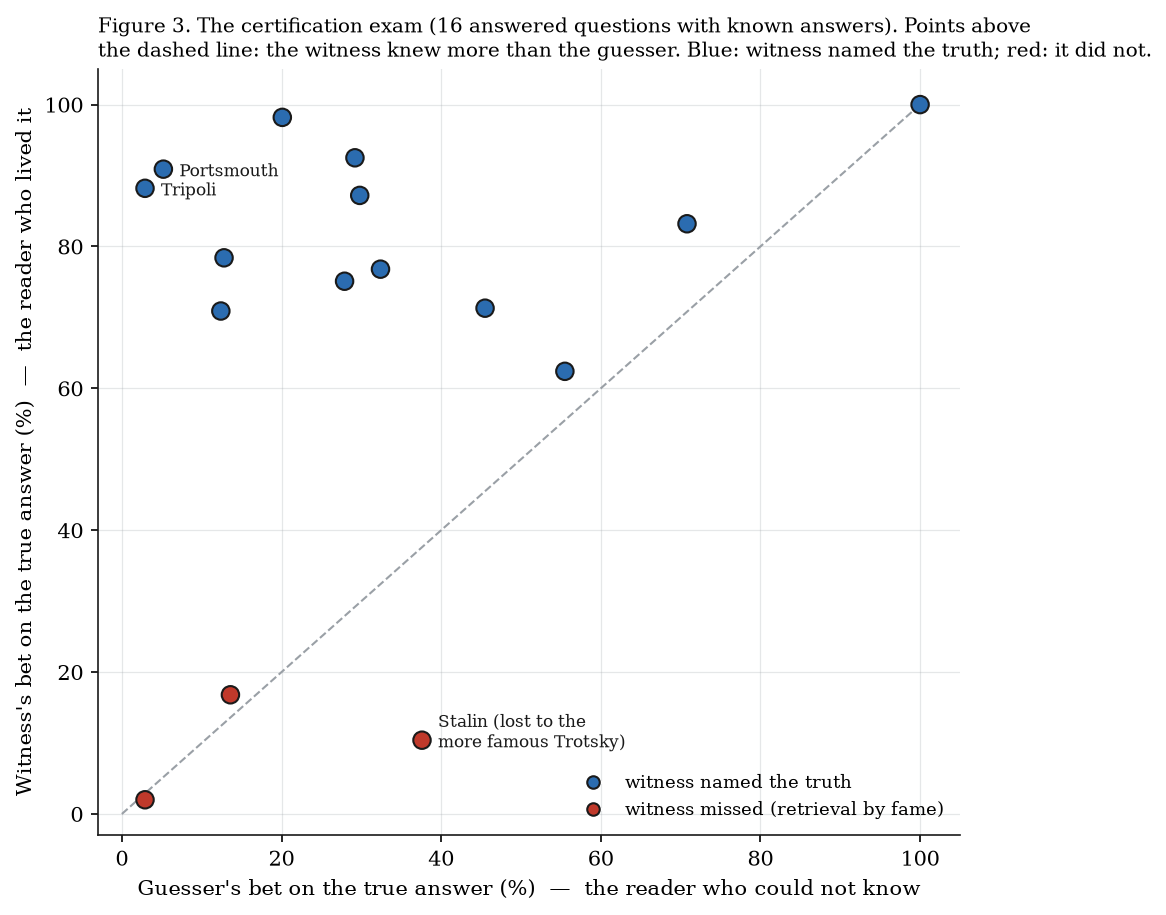
\includegraphics[width=.72\textwidth]{fig_exam.png}
\caption{The certification exam. Each point is one of the \NexamAnswered{} questions the meter agreed to
answer. The horizontal axis shows how much the guesser (the reader who could not know the event) bet on the
true answer; the vertical axis shows how much the witness (the reader who lived through it) bet on the same
answer. Points above the dashed line are questions where the witness knew more than the guesser --- almost
all of them. Blue points are questions where the witness named the truth; the three red points are the
failures, where a more famous rival drew the bet away (Stalin behind Trotsky, Bl\'eriot behind Latham).
Take-away: on questions with known answers, the later reader knows and the earlier reader guesses, which is
what a working instrument must show.}
\label{fig:exam}
\end{figure}

The fresh run passed. Take one question: ``it is 1906; the peace between Russia and Japan was signed last
year at\ldots'', with endings Portsmouth, Washington, Geneva, and The Hague. The 1900 guesser, for whom the
treaty had not happened, put \NportPre\% on Portsmouth and favored \NportGuess{} --- a reasonable guess. The
1913 witness put \NportPost\% on Portsmouth. Across all \NexamTotal{} questions the meter agreed to answer
\NexamAnswered{}, above the mark of \NbarAnswer{}; the witness named the truth in \NexamCorrect{} of those
\NexamAnswered{} ($\NexamCorrectPct\%$, mark \NbarCorrect{}); and the witness out-bet the guesser in
\NexamOutbet{} of \NexamAnswered{} ($\NexamOutbetPct\%$, mark \NbarOutbet{}). All three marks met. The meter
is certified in English.

One failure marks the instrument's limit and is worth keeping in view. Asked who ruled Russia after Lenin's
death, the 1929 reader answered \NstalinNames{}, putting only \NstalinPost\% on Stalin, the right answer. In
the Western press of the late 1920s Trotsky was by far the more written-about man, and these readers
retrieve by fame: set the truth beside a more famous rival and they can take the celebrity. This is the
failure mode of condition (iii), it is real, and it is why we ask only where the truth is the famous
version and flag the questions that break the rule.

That the exam can be failed is the point. The development run did fail it, on coverage, and forced the
scoring repair; the German and French runs fail it too (Section~\ref{sec:languages}). An instrument that
passes an exam it could have failed has earned something a plausible story has not.

\section{The twist: the frozen readers leak the future}\label{sec:leak}

The exam certifies that the witness knows and the guesser bets sensibly. It does not certify the premise
of condition (ii) --- that the guesser knows \emph{nothing} from after its cutoff. That premise is a claim
about how the training corpora were assembled, and corpora are assembled by imperfect filters. So we
tested it, behaviourally, on the models themselves.

The test asks for a date. Show the model a sentence naming an event --- ``The great war that engulfed
Europe began in the year'' --- and read off its probability over candidate years. A model that knows the
event concentrates on the true year; a model that does not spreads its bets. The \emph{date spike} is the
probability on the true year relative to the average on neighbouring years. The crucial step is
calibration: how big a spike is innocent? We answer with a \emph{fiction floor}: fifteen events we
invented ourselves --- the Treaty of Kesselheim, the Battle of Verronne, the novelist Aldous Brennt ---
each assigned a year no model can know, because it does not exist. On these the 1913 reader's spikes stay
at or below \NspikeNullNinetyFifthThirteen$\times$, and on nineteen famous events it genuinely studied
(Waterloo, the Franco-Prussian war) its median spike is \NspikeKnownMedThirteen$\times$. That brackets the
scale: near $1\times$ is ignorance, hundreds is memory.

\begin{figure}[t]\centering
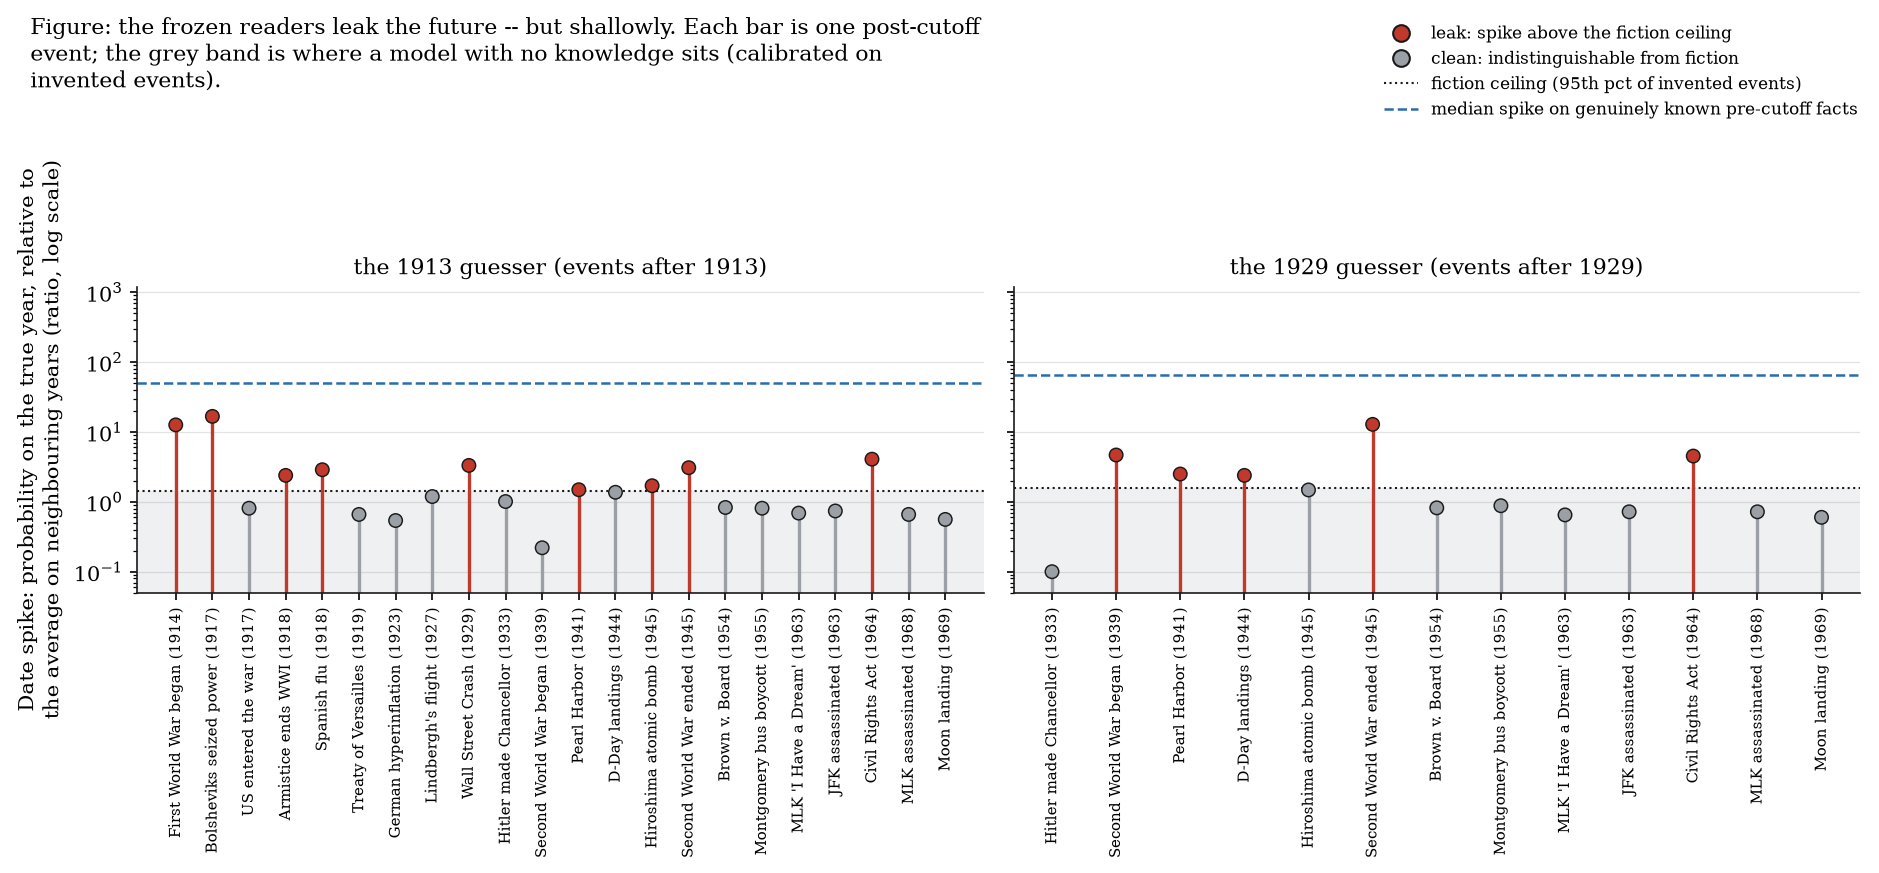
\includegraphics[width=.99\textwidth]{fig_leak_v5.png}
\caption{The leak, event by event. Each panel shows one frozen reader (left: the 1913 model; right: the
1929 model) asked to date events from \emph{after} its training cutoff --- events it should know nothing
about. The vertical axis is the date spike: the model's probability on the true year relative to the
average on neighbouring years, on a log scale. The grey band, bounded by the dotted line, is the fiction
ceiling: the 95th percentile of spikes on events we invented, i.e.\ the most a model can score knowing
nothing. The dashed blue line is the median spike on famous pre-cutoff facts the model genuinely studied.
Red points breach the ceiling: the model knows a date it should not. Grey points are indistinguishable
from fiction. Take-away: the leak is real but shallow and selective --- a handful of canonical dates
(the war, the revolution, the end of the Second World War, the Civil Rights Act) sit above the ceiling
yet far below real memory, while most of the future (Pearl Harbor for the 1913 reader, the moon landing,
the assassinations) stays dark.}
\label{fig:leak}
\end{figure}

The premise fails (Figure~\ref{fig:leak}; the full table is Appendix~\ref{app:audit}). The 1913 reader
dates the World War at \NspikeWWIThirteen$\times$ and the Bolshevik seizure of power at
\NspikeBolshThirteen$\times$ --- an order of magnitude above its fiction ceiling. It even dates the Civil
Rights Act of 1964, half a century past its cutoff, at \NspikeCRAThirteen$\times$. The 1929 reader dates
the end of the Second World War at \NspikeWWtwoEndTwentyNine$\times$ and its beginning at
\NspikeWWtwoBegTwentyNine$\times$. In all, \NleakCountThirteen{} of \NpostCountThirteen{} post-cutoff
events breach the 1913 reader's ceiling, and \NleakCountTwentyNine{} of \NpostCountTwentyNine{} breach
the 1929 reader's. Documents from after the cutoff --- enough of them to teach a handful of canonical
``event: year'' facts --- slipped through the date filter that built the corpora.

Three features of the leak matter for everything that follows. It is \emph{shallow}: every leaked spike
sits between the fiction ceiling and roughly a tenth of the known-fact median --- vague traces, not
studied history. It is \emph{selective}: the leak tracks how canonical a fact's dateline is, not how close
it is in time --- the 1913 reader leaks 1964's Civil Rights Act while staying dark on Pearl Harbor, and
both readers are at chance on the moon landing (\NspikeMoonThirteen$\times$ and
\NspikeMoonTwentyNine$\times$). And it is \emph{asymmetric in what it can corrupt}: a model that has
absorbed a stray sentence about the war knows \emph{that} the war came, which can inflate its apparent
foresight; but no stray sentence can make a knowing model bet wrong. Leakage fakes foresight; it cannot
fake blindness. That asymmetry is what the screen of the next section exploits.

The depth of the leak is worth one more probe, because ``knows the date'' overstates it. Asked in free
writing what became of the Tsar, the 1913 reader --- the same one that dates the revolution --- has him
exiled, not shot; asked who leads Germany after a lost war it has never heard of Ebert. The leaked traces
are datelines without content, the skeleton of an encyclopedia entry rather than the entry. This is why
the screen below asks not just \emph{does the guesser know the event} but \emph{does its bet lean toward
the truth} --- the conjunction, not the date alone, is what discredits a finding.

\section{The screen: telling foresight from leakage}\label{sec:screen}

The screen has three instruments, in increasing order of intimacy with the model, and a triage rule that
applies them to every finding in the paper.

\paragraph{The date spike is the primary signal.} It is behavioural, cheap, and calibrated against the
fiction floor, so it inherits no assumption about what the model ``should'' know. Its job is the first
question: does this guesser know that this event happened when it did? For each catastrophe we read the
guesser's probability on the true year against its own fiction floor. The war stands at \NdateWar\%
against the 1913 reader's floor of \NfloorThirteen\%; the revolution at \NdateRev\%; the fall of the
empires at \NdateEmp\%. But the hyperinflation sits at \NdateInfl\% --- below the floor; the 1913 reader
does not know the inflation happened. The 1900 reader puts \NdatePanic\% on 1907 for the panic: clean.
The 1929 reader puts \NdateDep\% on the crash year and \NdateNazi\% on 1933: clean on both. The
instrument that found the leak also certifies where the leak is not.

\paragraph{An internal probe reads memory against bluffing.} Output behaviour has a blind spot: a model
can \emph{sound} confident about a fact it is inventing. Our frozen readers do this constantly --- asked
to date the Treaty of Bordeaux, a treaty that does not exist, the 1929 reader puts \NbordeauxPeak\% of
its money on one specific year. Spoken confidence cannot separate such bluffs from memory
(Figure~\ref{fig:bluff}): among \NbluffTotal{} invented treaties, \NbluffN{} draw confident dates, while
the real Treaty of Portsmouth draws only \NportsmouthConf\%. So we go inside. A linear probe
\citep{alain2017} trained on the model's residual-stream activations --- real remembered facts against
invented ones --- reads \emph{retrieval versus confabulation} at an AUC of \NmeterAUC{}, and on the
confidence-matched hard cases (real memory versus confident bluff) the probe scores \NbluffProbeAUC{}
where output confidence manages \NbluffOutAUC{}. Trained only on knowns and inventions, it generalizes to
the categories it never saw: post-cutoff events the date test calls clean read \NmeterUnknown{} on the
probe ($n=\NmeterUnknownN$), and post-cutoff events the date test calls leaked read \NmeterLeaked{}
($n=\NmeterLeakedN$) --- independent confirmation, from inside the network, of the leak found outside.

\begin{figure}[t]\centering
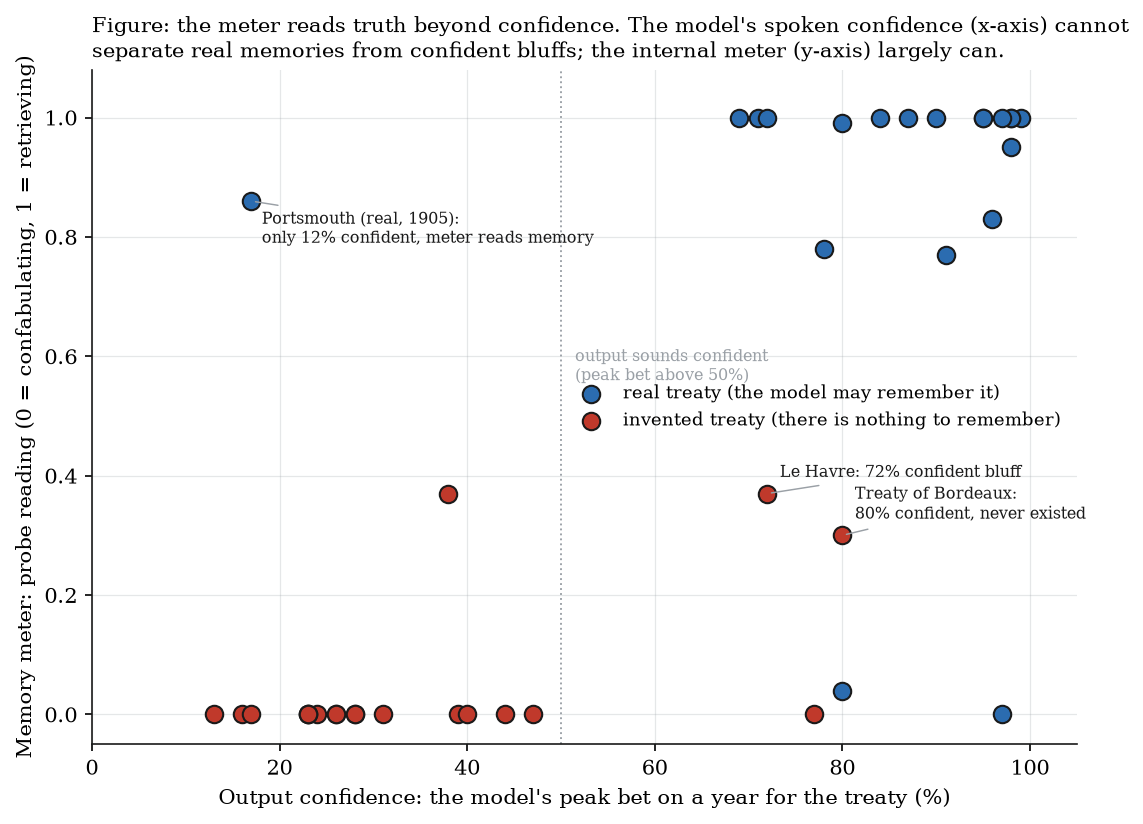
\includegraphics[width=.78\textwidth]{fig_bluff_v5.png}
\caption{The confident bluff, and the probe that catches it. Each point is one treaty put to the frozen
1929 reader. The horizontal axis shows the model's spoken confidence: its peak bet on a year for that
treaty, in percent. The vertical axis shows the internal memory meter: a linear probe on the model's
activations, reading 0 for confabulation and 1 for retrieval. Blue points are real treaties; red points
are treaties we invented, so there is nothing to remember. To the right of the dotted line the model
sounds sure of itself --- and red points reach there (the invented Treaty of Bordeaux draws an
\NbordeauxPeak\% bet), while a real memory (Portsmouth, 1905) can sound unsure at \NportsmouthConf\%.
The meter separates what the voice cannot: real treaties read high, invented ones read near zero.
Take-away: the model's stated confidence is no guide to whether it remembers; the internal probe largely
is.}
\label{fig:bluff}
\end{figure}

\paragraph{A causal check shows the probe reads storage, not style.} A correlational probe could be
reading some flavour of ``sounds real'' rather than memory itself. So we edited memory directly: a
rank-one weight edit in the style of \citet{meng2022} plants a specific date for a specific treaty into
one layer of the network, leaving every input byte unchanged. After the edit the model states the planted
year for all \NromeFakesN{} injected inventions --- the output cannot tell us which of them was truly
written into memory. The probe can: it flips to ``retrieval'' where the edit genuinely lodged
(\NromeProbeFlips{} of \NromeFakesN{}, plus the real-but-absent Treaty of Bj\"ork\"o, which flips from
\NbjorkoPreProbe{} to \NbjorkoPostProbe{}) and stays down where the edit merely forced the answer, while
un-edited controls hold still (real memories at \NromeCtrlReal\%, other inventions at \NromeCtrlFake).
Change the memory and the needle moves; force the answer and it does not (Figure~\ref{fig:rome}). A
two-model check closes the loop: trained separately on the 1913 and 1929 readers and shown the same
1914--1929 events, the two probes disagree exactly where they should --- events unknown to the earlier
reader and known to the later one shift from \NshiftCleanThirteen{} to \NshiftCleanTwentyNine{} (the
Lusitania: \NshiftLusitaniaThirteen{} to \NshiftLusitaniaTwentyNine{}), while shared knowns stay at
\NshiftKnownThirteen/\NshiftKnownTwentyNine{} and shared fictions at
\NshiftFictThirteen/\NshiftFictTwentyNine.

\begin{figure}[t]\centering
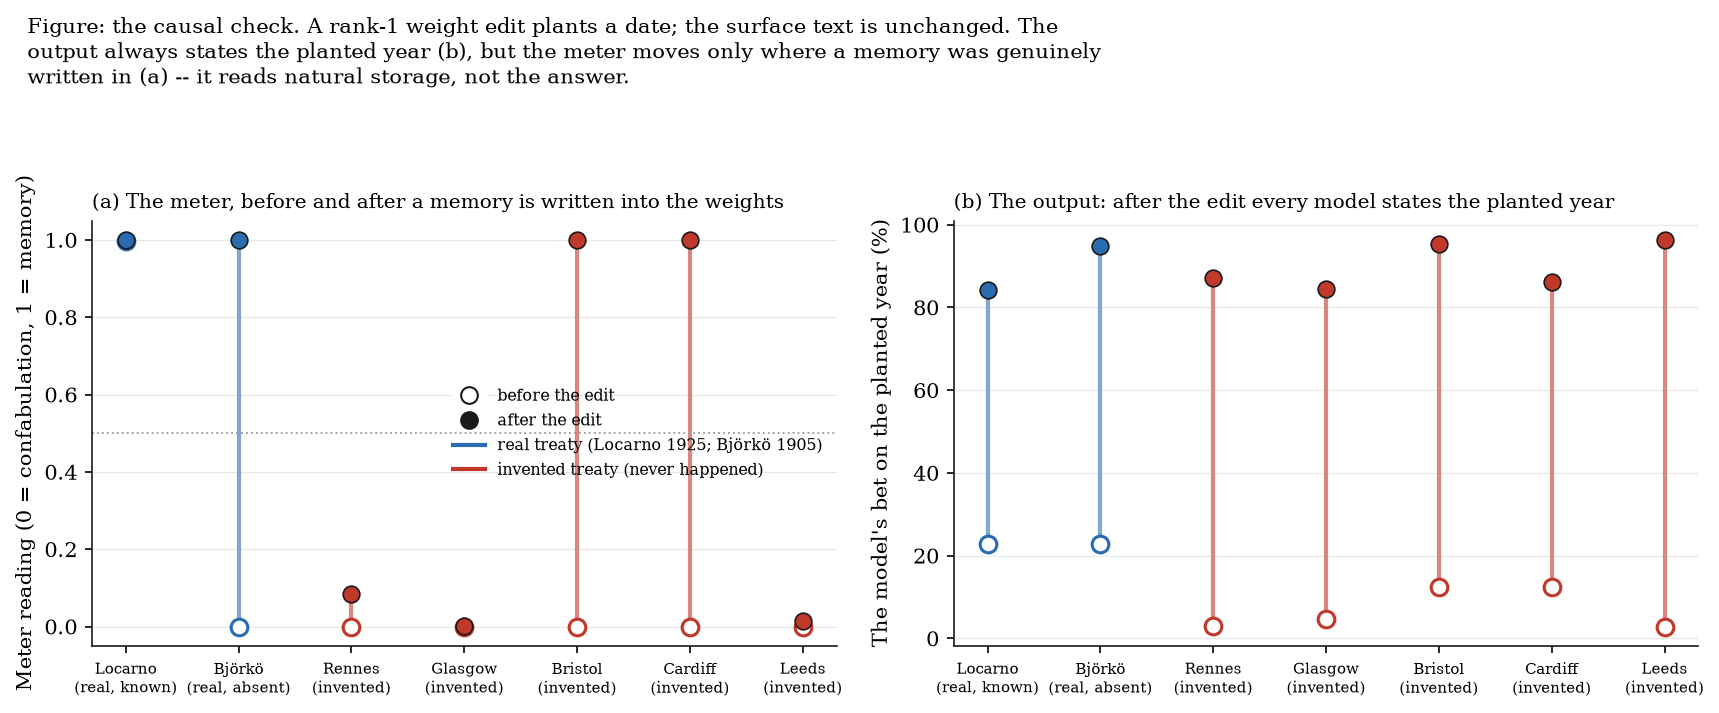
\includegraphics[width=.99\textwidth]{fig_rome_v5.png}
\caption{The causal check. Seven treaties are put to the frozen 1929 reader; for each, a rank-one weight
edit plants a date into layer 9 of the network, with the input text unchanged. Locarno (1925) and
Bj\"ork\"o (1905) are real treaties --- Locarno one the model already remembers, Bj\"ork\"o one it
provably does not; the other five are invented. Panel (b): after the edit, every model states the planted
year with high confidence --- the output is uninformative about what was truly stored. Panel (a): the
memory meter, read at layer 28, moves only where a memory genuinely lodged --- Bj\"ork\"o flips from
\NbjorkoPreProbe{} to \NbjorkoPostProbe{}, Bristol and Cardiff flip among the inventions, Rennes, Glasgow
and Leeds barely move despite producing the planted year, and the already-remembered Locarno stays at 1
throughout. Open circles: before the edit; filled circles: after. Blue: real treaties; red: invented
ones. Take-away: the probe reads naturally stored memory, not the answer the model was forced to give.}
\label{fig:rome}
\end{figure}

\paragraph{Honest bounds.} The probe is a specialist, not an oracle. Its known liability is a
\emph{realness} bias: a real but never-studied entity can read higher than an invented one --- familiarity
of the name, not memory of the fact. The bias is measurable, is largely removable by projecting the
realness direction out of the probe's feature space \citep{ravfogel2020}, and a residual remains; the
companion technical note documents both the correction and the residue at replication grade. For this
paper the probe therefore plays only the role no output test can play --- catching confident bluffs and
confirming the leak from inside --- while every verdict below rests on the calibrated behavioural test.
Both are pre-filters in the end: the gold standard is a search of the training corpus itself, which is
queued as the next step of this project (Section~\ref{sec:limits}).

\paragraph{The triage rule.} Every finding is now screened: flag it as \emph{suspect} if the guesser
breaches its fiction floor on the event's date \emph{and} its bets lean toward the true outcome (top bet
on the truth, or more than half its money there); keep it as \emph{clean} if either the guesser is
date-clean --- it does not know the event happened --- or it knows the event and still bets on the wrong
future, which leakage cannot produce. Of the \NgatePassed{} witness-certified findings,
\NgatedSafe{} come through clean and \NgatedSuspect{} are flagged (of \NtriageItems{} questions screened
in all, \NtriageSuspect{} are flagged; Appendix~\ref{app:audit} lists every verdict). The flagged three
are named in the next section, in the open.

\section{What was foreseen, what was not --- and what cannot be told apart from leakage}\label{sec:results}

We put the certified meter to \NnEvents{} catastrophes between 1907 and 1933, with several questions each.
The full funnel, stated once so the reader can weigh it: \NnMeasured{} questions have a witness; the meter
agreed to score \NnCovered{} of them (the rest fail the two-rule agreement test of Section~\ref{sec:gap});
the witness gate keeps \NgatePassed{} of those; and the contamination screen passes \NgatedSafe{} clean,
flagging \NgatedSuspect{}. Figure~\ref{fig:gaps} is the paper in one picture, and Table~\ref{tab:gaps}
lists the certified findings with their verdicts; Appendix~\ref{app:audit} accounts for every dropped and
flagged question.

\begin{figure}[t]\centering
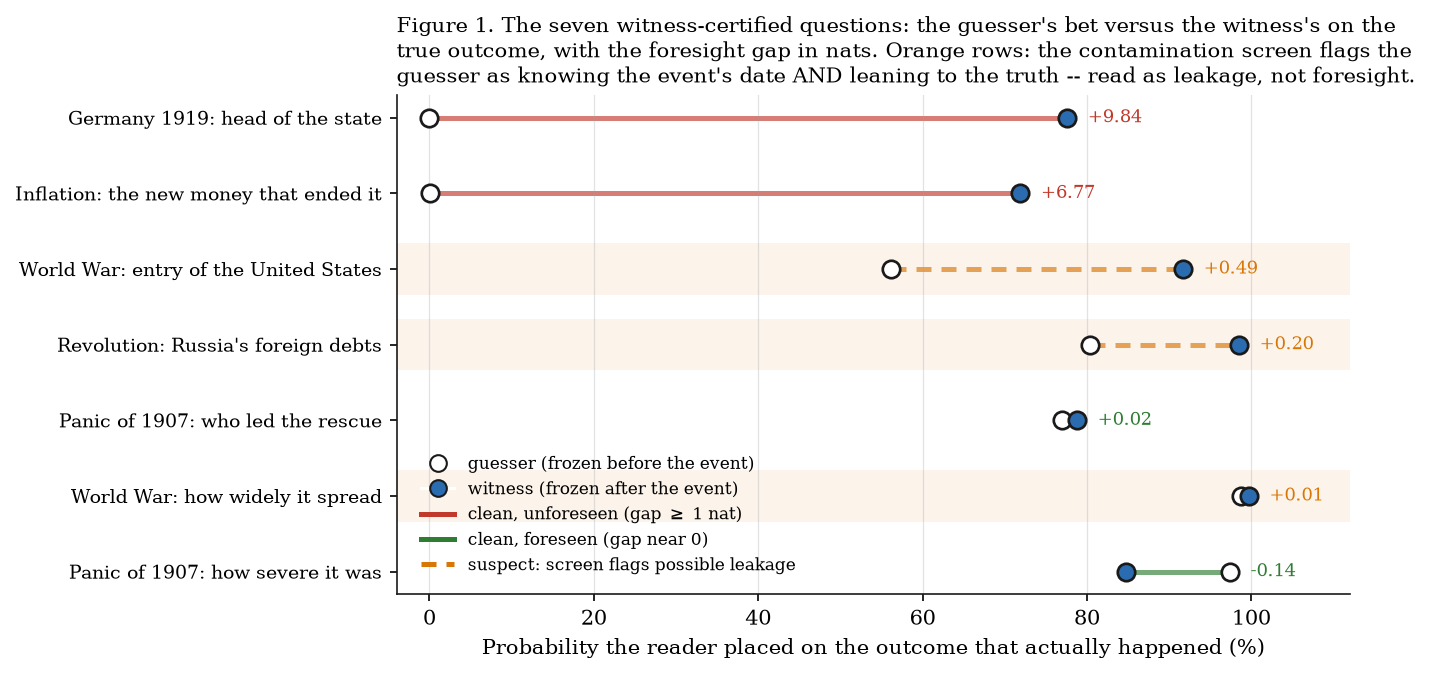
\includegraphics[width=.96\textwidth]{fig_gaps_v5.png}
\caption{The foresight gap, question by question, for the \NgatePassed{} witness-certified questions in
English. For each question the open circle is the guesser's bet on the outcome that in fact happened and
the filled blue circle is the witness's; the horizontal distance between them, labelled in nats, is the
foresight gap. Red lines are cleanly measured unforeseen outcomes (gap of one nat or more): only the
witness knew. Green lines are cleanly measured foreseen outcomes (gap near zero): the earlier reader found
the truth about as easily as the later one. Orange dashed lines on shaded rows are the findings the
contamination screen flags: the guesser knows the event's date (its bet on the true year breaches the
fiction floor) \emph{and} leans to the true outcome, so genuine foresight cannot be told apart from
leakage and we do not claim it. Take-away: the German republic and the new money that ended the inflation
were outside the pre-event picture by enormous margins; the panic of 1907 was inside it; and the three
questions where the pre-war reader seemed most prescient are exactly the ones its secret knowledge
discredits.}
\label{fig:gaps}
\end{figure}

\begin{table}[t]\centering\small
\begin{tabular}{p{4.9cm}ccr p{2.9cm}l}
\toprule
Question & Guesser & Witness & Gap & The guesser's memoir instead & Screen \\
\midrule
who headed the German state in 1919 & 0\% & 78\% & $+9.84$ & Kaiser Wilhelm & clean \\
the new money that ended the German inflation & 0\% & 72\% & $+6.77$ & Goldmark & clean \\
who joined the war against Germany in 1917 & 56\% & 92\% & $+0.49$ & the United States & \textbf{suspect} \\
what became of Russia's foreign debts & 80\% & 98\% & $+0.20$ & repudiated by the new rulers & \textbf{suspect} \\
who led the rescue in 1907 & 77\% & 79\% & $+0.02$ & Mister Morgan & clean \\
how widely the war spread & 99\% & 100\% & $+0.01$ & nearly every great power on earth & \textbf{suspect} \\
how severe the panic of 1907 was & 97\% & 85\% & $-0.14$ & sharper than any panic in memory & clean \\
\bottomrule
\end{tabular}
\caption{The witness-certified findings, in English. ``Guesser'' and ``witness'' are the probability each
reader placed on the ending that in fact happened; the gap is the guesser's surprise minus the witness's,
in nats. ``Screen'' reports the contamination triage: \emph{clean} means the guesser either does not know
the event's date or bets against the truth despite knowing it; \emph{suspect} means the guesser knows the
date and leans to the truth, so the apparent foresight may be leakage. Rows are ordered by gap.}
\label{tab:gaps}
\end{table}

Take the largest gap first, since it is now also the best-audited case. The question is who headed the
German state in 1919, with the endings President Ebert, Kaiser Wilhelm, Crown Prince Wilhelm, and Marshal
Hindenburg. The 1913 guesser, even after being told the war was lost, put essentially nothing on Ebert ---
about \NkaiserPreImplied\% --- and nearly all of it, \NkaiserPreBetP\%, went wrongly to the Kaiser. The
1929 witness put \NkaiserPost\% on Ebert. The guesser's surprise at the republic is about
\NkaiserSurpPre{} nats, the witness's about \NkaiserSurpPost{}, and the gap between them is \NkaiserGap{}
nats, the largest in the study. What makes the case airtight is that the screen \emph{did} find leakage
here --- the 1913 reader breaches its floor on the war's dateline (\NdateEmp\% on 1918 for the fall of
the empires) --- and the reader still bet everything on the Kaiser. A guesser that has absorbed stray
sentences about the war and \emph{still} cannot reach the republic is stronger evidence of
unforeseeability, not weaker: whatever leaked did not contain the future's content. A German republic was
not in the pre-war picture, not even the picture of a defeated Germany, not even with contaminated ink in
the training corpus.

One caveat attends the number, and we measured it rather than merely disclose it. ``President Ebert'' is
a name, and a 1913 reader might be blank on the man while conceiving the office. So we re-ran the
identical stems with offices in place of men: an elected president, the Kaiser on his throne, a general
with dictatorial power, a council of workmen and soldiers. This version cannot be certified as a gap ---
office-phrases pull the 1929 witness to the workers' councils of the post-war months (\NnfCouncilPost\%)
and the meter declines the question, in the 1919 and 1920 settings alike --- but the guesser's side,
which is what the caveat concerns, is unambiguous: told the war is lost, the 1913 reader bets
\NnfTwentyKaiserPre\% that the Kaiser still reigns and \NnfTwentyPresPre\% on an elected president. Nine
to one against the republic as an \emph{office}, not merely against the man; the free-writing evidence
agrees (no 1913 completion ever volunteers an elected head for a defeated Germany). The direction of the
flagship is not a name artifact. Its magnitude partly is: missing the office costs the guesser about
\NnfTwentySurpPre{} nats, missing the man about \NkaiserSurpPre{}. The honest statement of the flagship
is therefore double: the republic as a form of state was a nine-to-one underdog in the pre-war mind, and
the republic as it actually arrived --- with a saddler's son nobody had heard of at its head --- was
outside that mind entirely.

A claim of unforeseeability is a negative claim, and a negative can never be proven --- only bounded.
We bound this one the way an experimental physicist bounds an undiscovered particle: with an
instrument of demonstrated sensitivity that reads nothing. A free-association probe (say the bare
name, ask nothing, and measure which words rise in the model's next-word probabilities against
matched control names and a floor set by invented persons) was first \emph{calibrated by insertion}:
a memory of ``Ebert became president'', surgically written into the model's weights from three
sentences, drives the reading to \NebertAssocPlanted{} --- far above the detection floor of
\NassocFloor{}. Pointed at the real, unedited model, the same instrument reads \NebertAssocPres{} on
\emph{president} --- below zero --- and Ebert's warmest association of any kind sits at
\NebertAssocMax{}, still under the floor. The same probe, in the same model, lights up where
something is genuinely stored (it flags the model's leaked traces of interwar figures). So the
pre-war blank on the republic's first president is not ``we found nothing'': it is \emph{nothing,
down to the level of a detectable three-sentence trace}, from an instrument proven able to see one.
And the direction of every residual error is conservative: leakage can only manufacture foresight, so
whatever contamination survives our screens makes these gaps understatements.

The new money tells the same story more cleanly still. Asked what ended the inflation, the guesser
sensibly expects a ``Goldmark'', a gold-backed mark of the old kind, and is wrong; the Rentenmark, backed
by land, was a genuine invention, and the gap is \NinflendGap{} nats. Here the screen finds nothing at
all: the 1913 reader's bet on the inflation's date is \NdateInfl\%, \emph{below} its own fiction floor ---
it does not know the hyperinflation ever happened. This is the cleanest possible configuration: a guesser
provably ignorant of the event, missing the outcome by a factor of hundreds.

How large are these two gaps? We built a yardstick: \NmundaneN{} mundane changes across the same
between-cutoff windows --- elections, successions, conferences, ship launches, prizes, sporting and
technical firsts --- scored by the same meter under the same rules (\NmundaneGated{} pass the witness
gate; the fact list was vetted item by item). One
exclusion rule shapes the set: no pure name lotteries --- questions whose truth is the name of a private
individual with no pre-event public existence measure name-drawing, not the guessability of change, and
are excluded by rule; the names of kings and presidents stay, because a new officeholder's name is a
constrained public choice. The mundane median gap is \NmundaneMedian{} nats and the 90th percentile
\NmundaneNinety{}: ordinary between-cutoff change is mostly guessable. Ebert at \NkaiserGap{} and the
Rentenmark at \NinflendGap{} sit at the \NkaiserMundanePct th percentile of that distribution: all
\NmundaneGated{} ordinary changes were easier for the pre-event mind to reach. The sharpest comparison
is the yardstick's hardest item: naming the king of Norway, a country that did not exist as a kingdom
before 1905, costs the 1900 reader \NnorwayGap{} nats --- it bets on \NnorwayGuesserBet{}, the old union
king, exactly as the 1913 reader bets on the Kaiser. The German republic (\NkaiserGap{}) sits three and
a half nats above even that: the republic was harder to reach than the naming of a new country's new
king.

The panic of 1907 is the clean ``foreseen'' anchor --- and the screen matters for it in the opposite
direction. The 1900 reader bets \NpanicsevPre\% that the coming panic will be ``sharper than any panic in
memory'' (gap \NpanicsevGap) and \NpanicrescPre\% that ``Mister Morgan'' will lead the rescue (gap
\NpanicrescGap), essentially matching the witness. The screen certifies the reading: the 1900 model's bet
on the panic's date is \NdatePanic\%, far below its floor of \NfloorNineHundred\% --- it is provably not
remembering 1907; it is reasoning from the panics of 1893 and 1873. Financial panic was a genre the
American record had rehearsed to the point where a well-read mind of 1900 could write the next one in
advance, down to the name of the rescuer. That the panic reads as foreseen is not a free pass but a test
the instrument had to clear: panics were chosen in advance as the positive control, and a gauge that made
them look like bolts from the blue would have been wrong.

Now the retraction. In the previous draft of this paper, three more findings sat in the foreseen column,
and they were its most striking lines: the spread of the war to every great power (guesser
\NbreadthPre\%, gap \NbreadthGap), the entry of the United States (\NusentryPre\%, gap \NusentryGap), and
--- against the textbook account of the French bondholder's ruin --- the repudiation of Russia's foreign
debts (\NdebtsPre\%, gap \NdebtsGap). The screen flags all three. The 1913 guesser breaches its fiction
floor on the war's date by a factor of five (\NdateWar\% against \NfloorThirteen\%) and on the
revolution's by six (\NdateRev\%), and in each of these three questions its bets lean toward the true
outcome. That conjunction is precisely the signature leakage would leave, and no reading of the
probabilities can now distinguish a 1913 mind that truly saw a world war coming from a 1913 corpus with
stray sentences about one in it. We therefore claim nothing about these questions --- not that they were
foreseen, not that they were not. They are unmeasurable on the present models, and Section~\ref{sec:limits}
says what would make them measurable. The cost of this honesty is real: the paper loses its ``the war was
already in the pre-war picture'' headline. What it buys is the right to state the surviving findings
without an asterisk.

Finally, the witness gate's drops, one of which is a finding about the instrument. The fate of the Tsar
--- ``been put to death with all his family'' against ``been driven from his throne'' --- shows a gap of
\NtsarGap{} nats, but the \emph{witness} puts only \NtsarWitnessP\% on the truth and bets
``\NtsarWitnessBet'' itself. The question contains two truths: the Tsar was driven from his throne in
March 1917 \emph{and} shot in July 1918, and both readers reasonably prefer the earlier, more
written-about one. A gap anchored on a witness that will not name the outcome is not a measurement, and
we drop it (along with two smaller items; Appendix~\ref{app:audit}) rather than report a number the
design cannot support. The free-generation probe keeps what is real in the observation: prompted for the
aftermath of a lost war, the 1913 reader volunteers the Tsar's deposition in \NfreeTsarTh{} of
completions --- the fall was foreseeable --- but the murder in the cellar is a question our current
question-shape cannot cleanly ask.

\section{The memoir of the 1930s}\label{sec:memoir}

For the Great Depression and the Nazi seizure of power no witness model yet exists, because none is trained
past 1929. There is no gap to compute. What we can read is the 1929 reader's memoir of the years just ahead
--- its bets, set beside what happened (Figure~\ref{fig:memoir}, Table~\ref{tab:memoir}). And here the
contamination screen gives an unqualified verdict: the 1929 guesser's bet on the crash's date is
\NdateDep\% and on 1933 for the seizure of power \NdateNazi\% --- both below its fiction floor of
\NfloorTwentyNine\%. Whatever leaked into the 1929 corpus, the Depression and Hitler did not. Every
prediction in this section is a genuine guess.

\begin{figure}[t]\centering
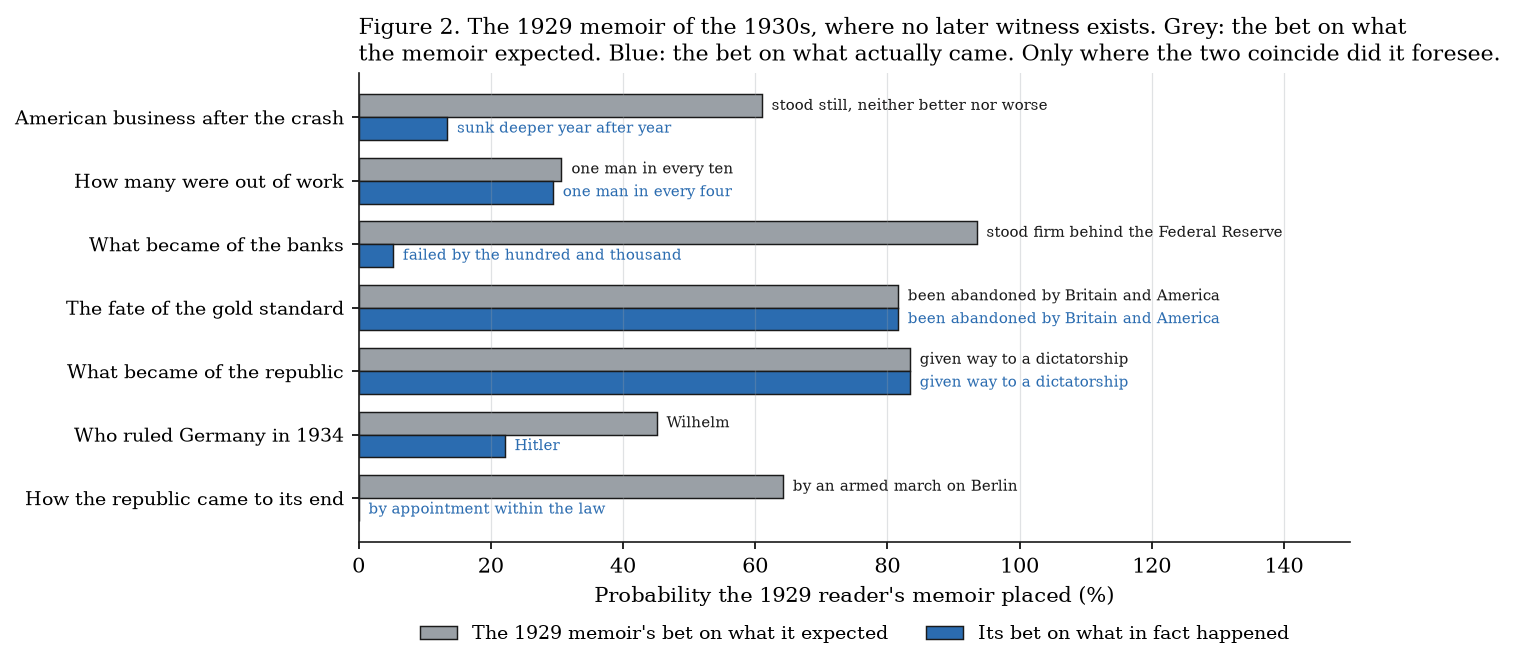
\includegraphics[width=.96\textwidth]{fig_memoir.png}
\caption{The 1929 reader's memoir of the 1930s, where no later witness exists. For each question the grey
bar is how much the memoir bet on the future it expected, the blue bar how much it bet on the future that
actually came; the text on each bar names the outcome. Where the two bars line up (the gold standard, the
slide into dictatorship) the memoir foresaw; where the grey bar towers over the blue (the course of
business, the fate of the banks, the ruler, the path to power) it expected the wrong thing. The
contamination screen certifies every row as a genuine guess: the 1929 reader is date-clean on both 1929
and 1933. Take-away: the misses are all the most recent precedent, reapplied.}
\label{fig:memoir}
\end{figure}

\begin{table}[t]\centering\small
\begin{tabular}{p{4.0cm}p{3.6cm}cp{3.1cm}c}
\toprule
Question & The 1929 memoir expects & Bet & What in fact happened & Bet on truth \\
\midrule
the course of American business after the crash & stood still, neither better nor worse & 61\% & sunk deeper year after year & 13\% \\
how many Americans were out of work & one man in every ten & 31\% & one man in every four & 29\% \\
what became of America's banks & stood firm behind the Federal Reserve & 94\% & failed by the hundred and thousand & 5\% \\
the fate of the gold standard & been abandoned by Britain and America & 82\% & been abandoned by Britain and America & 82\% \\
what became of the Weimar republic & given way to a dictatorship & 83\% & given way to a dictatorship & 83\% \\
who ruled Germany in 1934 & Wilhelm & 45\% & Hitler & 22\% \\
how the republic came to its end & by an armed march on Berlin & 64\% & by appointment within the law & 0\% \\
\bottomrule
\end{tabular}
\caption{The 1929 reader's memoir of the 1930s. No later reader exists, so there is no gap --- only the 1929
guesser's bets, beside the outcome that in fact followed and the bet the guesser placed on it. The screen
finds the 1929 reader date-clean on 1929 and 1933, so these are genuine ex-ante predictions.}
\label{tab:memoir}
\end{table}

The misses share one shape: the most recent precedent, applied again. American business, the memoir
expects, will have ``\NdepENbets'' four years after the crash ($\NdepENp\%$), the ordinary end of an
ordinary panic; in fact it sank deeper year on year, an ending the memoir gives \NdepENtruthP\%. The banks
will ``stand firm behind the Federal Reserve'', the new institution of 1913, trusted at \NdepBanksMemoir\%;
in fact they failed by the thousand. Power in Germany will be seized by an armed march on Berlin --- the
Kapp putsch of 1920, the Munich putsch of 1923, replayed --- and the master of Germany in 1934 will be a
Wilhelm before a Hitler. Each guess is the last crisis, reached for again.

Two bets land, and they are the two things the 1929 reader's own recent past had taught it. It expects the
Weimar republic to give way to a dictatorship (\NnaziDictMemoir\%), because its newspapers were already full
of government by emergency decree. And it finds it entirely likely that Britain and America will leave the
gold standard (\NdepGoldMemoir\%), because it had lived through exactly that between 1914 and 1925. Where the
future rhymed with the reader's own experience, the memoir was right; where the future broke new ground, it
reached for the nearest old thing.

\begin{quote}\small
A false alarm, caught by the rules. An earlier version of the ruler question seemed to have the 1929 memoir
putting \NfaOld\% on ``the leader of the National Socialists'' governing Germany in 1934 --- striking
foresight for 1929, when that party polled under three per cent. Rewritten with bare names --- Hitler,
Hindenburg, Wilhelm, Ludendorff --- the bet on Hitler falls to \NfaNew\%, no better than chance, and the
memoir's favorite is Wilhelm. The apparent foresight was the fluency of a stock phrase, not knowledge, and
it is exactly the error the two-rule scoring and the exam exist to catch.
\end{quote}

\section{The same test in German and French}\label{sec:languages}

The models read German and French as well as English, so we translated the exam and all the catastrophe
questions and ran the whole exercise again in each language, under the same rules and the same passing
marks. The first run failed in both languages: German answered only \NDEfirstAnswered{} of \NexamTotal{}
--- below the mark of \NbarAnswer{} --- and French answered \NFRfirstAnswered{} but out-bet the guesser in
only \NFRfirstOutbet{}, short of the third mark. The per-question autopsy found faults on our side of the
table, not the meter's: a German option declined in the wrong grammatical case; a German frame in which a
distractor was a second truth (the sea battle of 1905 was fought in the Strait of Korea as truly as at
Tsushima, and German usage says \emph{Koreastra\ss e}); a French truth missing its article; and a French
royal question whose bare-name options let the guesser be right on a name prior. So we made one declared
repair pass --- wordings only, the marks and the substance of every question untouched --- and re-ran once,
committing in advance to report the outcome either way. Because the questions had by then been seen, a pass
on the re-run certifies at a lower grade than the English held-out exam, and we label it so wherever the
numbers appear.

French passes the repaired run: \NFRexamAnswered{} of \NexamTotal{} answered (mark \NbarAnswer{}), the
witness right in \NFRexamCorrect{} of \NFRexamAnswered{}, out-betting the guesser in \NFRexamOutbet{} ---
all three marks met. German still fails, and its failure is now pure abstention: it answers only
\NDEexamAnswered{} questions, below the mark, but where it answers it is right \NDEexamCorrect{} times out
of \NDEexamAnswered{} and out-bets the guesser in \NDEexamOutbet{}. A meter that is precise when it speaks
but too often silent fails our bar honestly, and we do not lower the bar to let it through. The headline
claims accordingly rest on English; French now carries supporting weight at the repaired-run grade; German
remains supporting evidence without certification of its own.

They support the central result. The question of who headed Germany in 1919 is answered in all three
languages, and the answer is the same everywhere (Table~\ref{tab:crossling}): the guesser keeps the Kaiser,
the witness names Ebert, and the gap is large in every language.

\begin{table}[t]\centering\small
\begin{tabular}{lccr p{3.2cm}}
\toprule
Language & Guesser & Witness & Gap & The guesser's memoir keeps \\
\midrule
English & 0\% & 78\% & $+9.8$ & Kaiser Wilhelm \\
German & 0\% & 60\% & $+13.3$ & Kaiser Wilhelm \\
French & 0\% & 18\% & $+5.7$ & le Kaiser Guillaume \\
\bottomrule
\end{tabular}
\caption{The flagship question in three languages. The guesser's bet on the republic, the witness's bet, and
the gap in nats. The guesser keeps a monarch in every language; the gap is the German republic's distance
from the pre-war picture, and it is large everywhere.}
\label{tab:crossling}
\end{table}

The three languages also show something no single one could. Asked how American business fared in the four
years after the crash, the French memoir bets \NdepFRp\% on \emph{\NdepFRbets} --- recovered, as after every
panic --- while the German memoir bets \NdepDEp\% on \emph{\NdepDEbets} --- sunk deeper year on year. The
German memoir is the one that gets it right, and the likely reason is memory: the German 1920s, with their
inflation and slumps, had taught the German-language press what a collapse can be, while the French press
remembered recoveries. Each language forecasts from its own national memory. No survey taken in 1929 could
have recovered that.

\section{What the instrument cannot do}\label{sec:limits}

Five limits bound the claims, and we state them rather than bury them.

First, and foremost, the frozen readers are not perfectly frozen, and the screen is a filter, not a proof.
The date-spike test rests on one canonical phrasing per event, and phrasing matters at the margin; the
internal probe carries a known realness bias with a documented correction and a residue; and both are
pre-filters whose verdicts should ultimately be confirmed against the training corpus itself. That corpus
search --- locate the offending post-cutoff documents, identify the sources that carried them, and repair
the date filter that admitted them --- is queued, and it enables the real fix: retraining the readers on
verifiably clean corpora (at 1913, 1929, and, for the first time, 1938, which would turn the memoir of
Section~\ref{sec:memoir} into measured gaps). The date-spike test then doubles as the acceptance gate: a
clean retrain must put every leaked event back under the fiction ceiling. Until then, the three flagged
findings stay unmeasured, and the clean findings rest on the screen's asymmetry --- leakage cannot
manufacture a guesser that bets against a truth it knows.

Second, coverage is partial by design. The meter answered \NnCovered{} of the \NnMeasured{} questions with
a witness and declined the rest, because the two scoring rules disagreed on them; the witness gate then
dropped \NgateDropped{} more. Refusal is a feature --- it is what keeps the meter from scoring questions
where wording, not knowledge, would decide --- but it means the results describe the questions the
instrument could score fairly, not a random sample of all questions. We read the answered set, not a
census.

Third, retrieval by fame is a real failure mode, not a hypothetical one. The exam caught it (Stalin behind
Trotsky), and it would bias any question that set the truth beside a more famous rival. The flagship
carried a related caveat --- ``President Ebert'' is a name --- and Section~\ref{sec:results} reports the
name-free measurement that resolves it: the office was a nine-to-one underdog to the pre-war reader, so
the finding's direction survives name-free, while the headline magnitude should be read as the distance
to the republic \emph{as it arrived}, man and all. The name-free version itself illustrates the
instrument's limits: it loses its witness (the 1929 reader reads post-war Germany as council-governed and
the meter declines), so it is reported as a guesser-side robustness check, not as a certified gap.

Fourth, the two post-1929 events have no witness. The Depression and the Nazi seizure are read only as the
1929 memoir, with no later reader to anchor the gap, so for them we report the guesser's bets beside
history and claim no measured gap. A reader trained to 1938 would close this, and is the declared next
step.

Fifth, certification is graded by language. English is certified on a held-out exam. French passes only a
repaired run --- wordings corrected after one look at the results, marks unchanged, one pass by declared
protocol --- which is a real but weaker credential, and it is disclosed wherever French numbers appear.
German remains uncertified: on the repaired run it is right in all \NDEexamAnswered{} of the questions it
answers and out-bets the guesser in \NDEexamOutbet{} of them, but it answers too few. Its agreement with
the English results is supporting evidence, not independent confirmation, until its coverage is solved.

None of these overturns the central reading, because that reading rests on English questions the meter
answered, the exam certified, the witness gate anchored, and the contamination screen passed. But each
marks a place where the instrument is still short of what one would want, and where more work would
sharpen it.

\section{What the measurements change}\label{sec:implications}

Return to \citet{barro2006}. The rare-disaster account of the equity premium reads a disaster probability
off the realized twentieth century and attributes it, before the fact, to investors. Our measurements
speak to both halves of that move, but with different force than a naive reading would have given them.

On the support half --- were the catastrophes inside the set of futures contemporaries could conceive? ---
our evidence is narrower than we once believed, and we say so. The strongest apparent instances of
specific foresight (the war's spread, America's entry, Russia's default) are precisely the ones our
contamination screen disqualified. What survives is evidence about \emph{kind} rather than \emph{instance}:
the panic of 1907 was written in advance by a provably clean 1900 reader, down to its rescuer; the
selection arm (Appendix~\ref{app:selection}) shows the pre-event readers preferring true anatomies of
catastrophe to matched false ones wherever catastrophe was a rehearsed genre; and the memoir's correct
calls --- dictatorship, the end of gold --- are the rehearsed futures. The ``nobody could imagine it''
defense of low pre-1914 risk premia is therefore weakened but no longer refuted by our strongest lines:
on the specific July-1914 question our instrument now honestly abstains. What we can still reject is the
strong claim that the era's catastrophes were beyond the record's imagination in kind: panics, wars,
inflations, and fallen dynasties were all in the repertoire.

On the weighting half the evidence hardened, because it runs through the findings the screen certified
rather than the ones it removed. Everywhere we can measure cleanly, the pre-event mind put its probability
on the branch the last crisis had carved: a gold-backed mark for the next stable money, a Morgan for the
next rescue, a putsch for the next seizure of power, a recovery for the next depression --- and, in the
two cases where the future broke with all precedent, it missed by \NkaiserGap{} and \NinflendGap{} nats,
the \NkaiserMundanePct th percentile of a \NmundaneN-item yardstick of ordinary change. That is the
availability heuristic
\citep{tversky1973} read out of the written record of an age rather than a laboratory, and it is the
belief distortion that diagnostic-expectations theory \citep{bordalo2018,gennaioli2018} places at the
center of financial fragility. Models of time-varying disaster premia \citep{gabaix2012,wachter2013}
acquire a state variable that can be read decade by decade: perceived tail risk should load on how recent
and how vivid the last precedent was, and time-locked readers make that loading measurable. For the
peso-problem tradition \citep{krasker1980} the method supplies the missing observable --- the state that
is in minds but not in samples --- read out of the minds directly, together with the audit that says when
the reading can be trusted.

The methodological contribution runs beyond this paper's question. Detecting what a language model
secretly knows is an active literature: membership-inference tests read training-set membership off token
probabilities \citep{shi2024}, ``time-travel'' probes elicit memorized benchmark data \citep{golchin2024},
effective-cutoff studies show that a model's real knowledge horizon rarely matches its nominal one
\citep{cheng2024} --- by now a commodity technique, with live public benchmarks probing commercial
models' effective cutoffs against fabricated-event controls\footnote{E.g.\ the knowledge-cutoff
benchmark at \texttt{apoorvumang.github.io/knowledge-cutoff} (12 models, 330 unforecastable events,
fabricated-event controls; accessed July 2026).} --- and calibration work shows models partly know
what they know \citep{kadavath2022}. We
add three things that inference from purpose-built historical models specifically needs: a
\emph{fiction floor} --- calibrating every knowledge test against events invented so that ignorance has a
measured signature; a \emph{causal validation} of internal probes by direct memory editing, so the probe
is shown to read storage rather than style; and \emph{contamination-aware screening} --- a triage that
uses the direction of the bias to salvage the inferences leakage cannot have produced, rather than
discarding the instrument wholesale. Note what the problem is not: it is not hallucination, the
confidently wrong answer. Our problem is the mirror image --- the confidently \emph{right} answer about a
forbidden fact --- and it is the harder one to see, because it looks like success.

\section{Conclusion}\label{sec:conclusion}

Foreseeability can be measured, once you build a gauge that does not already know the ending --- and once
you check, rather than assume, that it does not. Frozen readers, asked for memoirs rather than prophecies,
certified by an exam, anchored by witnesses, and audited for leaks, give one number per catastrophe: how
much harder the truth was for the mind that came before than for the mind that came after. By those
numbers, the early twentieth century's catastrophes were thinkable in kind --- the panic read, to a
provably clean reader of 1900, about as easily as it read to a reader who lived it --- but the particular
new things were not: a republic in Germany and a land-backed currency sat further outside the pre-event
picture than anything else we measured, and the 1929 mind forecast the 1930s by its own most recent
crisis and missed, except where the future rhymed with its past. The failure of the age was less one of
imagination than of weighting, and that failure was regular enough to measure.

The audit is not a caveat to that story; it is half of it. The same models that measure history's
foresight turned out to be quietly remembering fragments of their own future, and the paper's claims
survive only because the leak's direction could be turned against it: contamination can counterfeit a
prophet, but not a blind man. The tools that did this --- the fiction floor, the internal memory meter
validated by editing memories into the weights, the triage rule --- travel to any study that reads the
past out of a time-locked model. The next steps are mechanical and declared: find the leaked documents in
the corpus, repair the filter, retrain clean readers at 1913, 1929, and 1938, and let the date-spike test
certify the fix --- every leaked event back under the fiction ceiling. A clean 1913 reader would let us
finally ask whether the war was foreseeable; a 1938 reader would turn the memoir of the Depression and of
Hitler into measured gaps. The instrument found its own flaw, measured it, and worked around it; the
repaired version gets to answer the questions this one had to decline.

\begin{thebibliography}{99}
\bibitem[Alain and Bengio(2017)]{alain2017} Alain, Guillaume, and Yoshua Bengio. 2017. ``Understanding
Intermediate Layers Using Linear Classifier Probes.'' arXiv:1610.01644.
\bibitem[Angell(1910)]{angell1910} Angell, Norman. 1910. \emph{The Great Illusion}. London: Heinemann.
\bibitem[Barro(2006)]{barro2006} Barro, Robert J. 2006. ``Rare Disasters and Asset Markets in the Twentieth
Century.'' \emph{Quarterly Journal of Economics} 121(3): 823--866.
\bibitem[Barro and Urs\'ua(2008)]{barroursua2008} Barro, Robert J., and Jos\'e F. Urs\'ua. 2008.
``Macroeconomic Crises since 1870.'' \emph{Brookings Papers on Economic Activity} 39(1): 255--350.
\bibitem[Bloch(1899)]{bloch1899} Bloch, Ivan S. 1899. \emph{Is War Now Impossible?} London: Grant Richards.
\bibitem[Bordalo et al.(2018)]{bordalo2018} Bordalo, Pedro, Nicola Gennaioli, and Andrei Shleifer. 2018.
``Diagnostic Expectations and Credit Cycles.'' \emph{Journal of Finance} 73(1): 199--227.
\bibitem[Bruner and Carr(2007)]{bruner2007} Bruner, Robert F., and Sean D. Carr. 2007. \emph{The Panic of
1907}. Hoboken: Wiley.
\bibitem[Cheng et al.(2024)]{cheng2024} Cheng, Jeffrey, Marc Marone, Orion Weller, Dawn Lawrie, Daniel
Khashabi, and Benjamin Van Durme. 2024. ``Dated Data: Tracing Knowledge Cutoffs in Large Language
Models.'' \emph{Conference on Language Modeling (COLM)}.
\bibitem[Clark(2012)]{clark2012} Clark, Christopher. 2012. \emph{The Sleepwalkers: How Europe Went to War in
1914}. London: Allen Lane.
\bibitem[Evans(2003)]{evans2003} Evans, Richard J. 2003. \emph{The Coming of the Third Reich}. London: Allen
Lane.
\bibitem[Ferguson(2006)]{ferguson2006} Ferguson, Niall. 2006. ``Political Risk and the International Bond
Market between the 1848 Revolution and the Outbreak of the First World War.'' \emph{Economic History Review}
59(1): 70--112.
\bibitem[Fisher(1930)]{fisher1930} Fisher, Irving. 1930. \emph{The Stock Market Crash---and After}. New
York: Macmillan.
\bibitem[Gabaix(2012)]{gabaix2012} Gabaix, Xavier. 2012. ``Variable Rare Disasters: An Exactly Solved
Framework for Ten Puzzles in Macro-Finance.'' \emph{Quarterly Journal of Economics} 127(2): 645--700.
\bibitem[Galbraith(1955)]{galbraith1955} Galbraith, John Kenneth. 1955. \emph{The Great Crash, 1929}.
Boston: Houghton Mifflin.
\bibitem[Gennaioli and Shleifer(2018)]{gennaioli2018} Gennaioli, Nicola, and Andrei Shleifer. 2018. \emph{A
Crisis of Beliefs: Investor Psychology and Financial Fragility}. Princeton: Princeton University Press.
\bibitem[Gentzkow et al.(2019)]{gentzkow2019} Gentzkow, Matthew, Bryan Kelly, and Matt Taddy. 2019. ``Text
as Data.'' \emph{Journal of Economic Literature} 57(3): 535--574.
\bibitem[Golchin and Surdeanu(2024)]{golchin2024} Golchin, Shahriar, and Mihai Surdeanu. 2024. ``Time
Travel in LLMs: Tracing Data Contamination in Large Language Models.'' \emph{International Conference on
Learning Representations (ICLR)}.
\bibitem[Kadavath et al.(2022)]{kadavath2022} Kadavath, Saurav, et al. 2022. ``Language Models (Mostly)
Know What They Know.'' arXiv:2207.05221.
\bibitem[Keynes(1919)]{keynes1919} Keynes, John Maynard. 1919. \emph{The Economic Consequences of the
Peace}. London: Macmillan.
\bibitem[Krasker(1980)]{krasker1980} Krasker, William S. 1980. ``The `Peso Problem' in Testing the
Efficiency of Forward Exchange Markets.'' \emph{Journal of Monetary Economics} 6(2): 269--276.
\bibitem[Kuran(1991)]{kuran1991} Kuran, Timur. 1991. ``Now Out of Never: The Element of Surprise in the East
European Revolution of 1989.'' \emph{World Politics} 44(1): 7--48.
\bibitem[Meng et al.(2022)]{meng2022} Meng, Kevin, David Bau, Alex Andonian, and Yonatan Belinkov. 2022.
``Locating and Editing Factual Associations in GPT.'' \emph{Advances in Neural Information Processing
Systems} 35.
\bibitem[Ravfogel et al.(2020)]{ravfogel2020} Ravfogel, Shauli, Yanai Elazar, Hila Gonen, Michael Twiton,
and Yoav Goldberg. 2020. ``Null It Out: Guarding Protected Attributes by Iterative Nullspace Projection.''
\emph{Proceedings of ACL}: 7237--7256.
\bibitem[Rietz(1988)]{rietz1988} Rietz, Thomas A. 1988. ``The Equity Risk Premium: A Solution.''
\emph{Journal of Monetary Economics} 22(1): 117--131.
\bibitem[Shi et al.(2024)]{shi2024} Shi, Weijia, Anirudh Ajith, Mengzhou Xia, Yangsibo Huang, Daogao Liu,
Terra Blevins, Danqi Chen, and Luke Zettlemoyer. 2024. ``Detecting Pretraining Data from Large Language
Models.'' \emph{International Conference on Learning Representations (ICLR)}.
\bibitem[Taleb(2007)]{taleb2007} Taleb, Nassim Nicholas. 2007. \emph{The Black Swan}. New York: Random House.
\bibitem[Tetlock(2005)]{tetlock2005} Tetlock, Philip E. 2005. \emph{Expert Political Judgment}. Princeton:
Princeton University Press.
\bibitem[Turner(1996)]{turner1996} Turner, Henry Ashby. 1996. \emph{Hitler's Thirty Days to Power: January
1933}. Reading, MA: Addison-Wesley.
\bibitem[Tversky and Kahneman(1973)]{tversky1973} Tversky, Amos, and Daniel Kahneman. 1973. ``Availability:
A Heuristic for Judging Frequency and Probability.'' \emph{Cognitive Psychology} 5(2): 207--232.
\bibitem[Wachter(2013)]{wachter2013} Wachter, Jessica A. 2013. ``Can Time-Varying Risk of Rare Disasters
Explain Aggregate Stock Market Volatility?'' \emph{Journal of Finance} 68(3): 987--1035.
\bibitem[Zweig(1942)]{zweig1942} Zweig, Stefan. 1942. \emph{The World of Yesterday}. Stockholm:
Bermann-Fischer.
\end{thebibliography}

\clearpage
\appendix
\renewcommand{\thesection}{\Alph{section}}

\section{The exam in full}\label{app:exam}
Table~\ref{tab:exam} lists all \NexamTotal{} held-out questions. For each, ``guesser'' is the probability
the reader frozen before the event placed on the true answer, ``witness'' the probability the reader frozen
after placed on it. ``Answered'' records whether the two scoring rules agreed enough for the meter to score
the question; ``witness right'' whether the witness named the truth. The English run met all three
pre-registered marks: \NexamAnswered{} answered (mark \NbarAnswer{}), witness right in $\NexamCorrectPct\%$
of answered (mark \NbarCorrect{}), witness out-bets the guesser in $\NexamOutbetPct\%$ (mark \NbarOutbet{}).
Every prompt and every ending is in \texttt{results/certify\_chronicle\_heldout.json}; the development run
that set the scoring rule is in \texttt{results/certify\_chronicle.json}.

\begin{table}[h]\centering\small
\begin{tabular}{p{6.6cm}cccc}
\toprule
Question & Guesser & Witness & Answered? & Witness right? \\
\midrule
The decisive sea battle of the Russo-Japanese war & 14\% & 17\% & yes & no \\
Where the Russo-Japanese peace was signed (1905) & 5\% & 91\% & yes & yes \\
Who succeeded to the British throne (1910) & 71\% & 83\% & yes & yes \\
The warship that renamed a class (1906) & 29\% & 92\% & yes & yes \\
Who first flew across the Channel (1909) & 3\% & 2\% & yes & no \\
The country of the 1908 revolution & 56\% & 62\% & yes & yes \\
Who seized Tripoli from the Ottomans (1911) & 3\% & 88\% & yes & yes \\
The isthmus the canal finally crossed & 12\% & 53\% & declined & -- \\
The form China took after 1911 & 12\% & 71\% & yes & yes \\
The fortress of the great 1916 battle & 32\% & 77\% & yes & yes \\
The largest naval battle of the war (1916) & 13\% & 78\% & yes & yes \\
The month the war ended (1918) & 28\% & 75\% & yes & yes \\
The town of the 1925 treaty & 30\% & 87\% & yes & yes \\
Who named the 1924 reparations plan & 20\% & 98\% & yes & yes \\
Who ruled Russia after Lenin & 38\% & 10\% & yes & no \\
The city of the 1921--22 naval conference & 46\% & 71\% & yes & yes \\
What became of Germany's colonies & 0\% & 32\% & declined & -- \\
What Austria became after 1918 & 18\% & 23\% & declined & -- \\
The fate of the surrendered German fleet & 3\% & 1\% & declined & -- \\
What women won after the war & 100\% & 100\% & yes & yes \\
\bottomrule
\end{tabular}
\caption{The held-out certification exam, all \NexamTotal{} questions. Guesser and witness are the bets on
the true answer; a question is ``declined'' when the two scoring rules disagree on the winner.}
\label{tab:exam}
\end{table}

\section{The contamination audit in full}\label{app:audit}

\paragraph{The leak, event by event.} Table~\ref{tab:spike} gives the date spike of both base-model
readers on every test event. The spike is the model's probability on the true year relative to the average
probability on neighbouring years; a model that knows nothing scores near $1\times$ (95th percentile on
invented events: \NspikeNullNinetyFifthThirteen$\times$ for the 1913 reader,
\NspikeNullNinetyFifthTwentyNine$\times$ for the 1929 reader), and a model that studied a fact scores in
the tens to hundreds (median on famous pre-cutoff facts: \NspikeKnownMedThirteen$\times$ and
\NspikeKnownMedTwentyNine$\times$ respectively). Bold entries breach the reader's own fiction ceiling on a
post-cutoff event: leaks. Note the pattern: the leaks concentrate on facts with canonical datelines (the
war, the revolution, the end of the Second World War, the Civil Rights Act of 1964) and skip more recent
but less dateline-shaped events entirely.

\begin{table}[h]\centering\small
\begin{tabular}{lc rr}
\toprule
Event & Year & Ranke-1913 & Ranke-1929 \\
\midrule
First World War began & 1914 & \textbf{13$\times$} & 943$\times$ \\
Bolsheviks seized power & 1917 & \textbf{17$\times$} & 89$\times$ \\
US entered the war & 1917 & 0.8$\times$ & 142$\times$ \\
Armistice ends WWI & 1918 & \textbf{2.4$\times$} & 35$\times$ \\
Spanish flu & 1918 & \textbf{2.9$\times$} & 325$\times$ \\
Treaty of Versailles & 1919 & 0.7$\times$ & 366$\times$ \\
German hyperinflation & 1923 & 0.5$\times$ & 2.7$\times$ \\
Lindbergh's flight & 1927 & 1.2$\times$ & 0.1$\times$ \\
Wall Street Crash & 1929 & \textbf{3.3$\times$} & 1.1$\times$ \\
Hitler made Chancellor & 1933 & 1.0$\times$ & 0.1$\times$ \\
Second World War began & 1939 & 0.2$\times$ & \textbf{4.7$\times$} \\
Pearl Harbor & 1941 & \textbf{1.5$\times$} & \textbf{2.5$\times$} \\
D-Day landings & 1944 & 1.4$\times$ & \textbf{2.4$\times$} \\
Hiroshima atomic bomb & 1945 & \textbf{1.7$\times$} & 1.5$\times$ \\
Second World War ended & 1945 & \textbf{3.1$\times$} & \textbf{13$\times$} \\
Brown v. Board & 1954 & 0.8$\times$ & 0.8$\times$ \\
Montgomery bus boycott & 1955 & 0.8$\times$ & 0.9$\times$ \\
MLK 'I Have a Dream' & 1963 & 0.7$\times$ & 0.7$\times$ \\
JFK assassinated & 1963 & 0.7$\times$ & 0.7$\times$ \\
Civil Rights Act & 1964 & \textbf{4.1$\times$} & \textbf{4.5$\times$} \\
MLK assassinated & 1968 & 0.7$\times$ & 0.7$\times$ \\
Moon landing & 1969 & 0.6$\times$ & 0.6$\times$ \\
\bottomrule
\end{tabular}
\caption{The date-spike audit of both frozen readers, all test events, base models. Entries are spike
ratios; bold = above that reader's fiction ceiling for an event after its cutoff (a leak). Events before a
reader's cutoff are real knowledge and shown for scale.}
\label{tab:spike}
\end{table}

\paragraph{The triage, question by question.} Table~\ref{tab:triage} applies the screen of
Section~\ref{sec:screen} to all \NtriageItems{} catastrophe questions with a witness: the guesser's bet on
the event's true year, its fiction floor, whether that constitutes a leak, whether the guesser's bets lean
toward the true outcome, and the verdict. \NtriageSuspect{} of \NtriageItems{} are flagged suspect ---
every one a ``foreseen'' World-War, revolution, or influenza item read by the 1913 guesser. The memoir
questions of Section~\ref{sec:memoir} are all read by a 1929 guesser that is date-clean on 1929 and 1933
(bets of \NdateDep\% and \NdateNazi\% against a floor of \NfloorTwentyNine\%) and are not tabulated.

\begin{table}[h]\centering\small
\begin{tabular}{p{4.9cm} c rr cc l}
\toprule
Question & Guesser & \multicolumn{1}{c}{$P$(yr)} & \multicolumn{1}{c}{floor} & Leak? & Leans truth? & Verdict \\
\midrule
who joined the war against Germany in 1917 & 1913 & 44\% & 8.1\% & yes & yes & \textbf{suspect} \\
how long the war lasted & 1913 & 44\% & 8.1\% & yes & yes & \textbf{suspect} \\
what became of Russia's foreign debts & 1913 & 51\% & 8.1\% & yes & yes & \textbf{suspect} \\
how widely the war spread & 1913 & 44\% & 8.1\% & yes & yes & \textbf{suspect} \\
how many the pandemic killed & 1913 & 15\% & 8.1\% & yes & yes & \textbf{suspect} \\
whether medicine found a remedy & 1913 & 15\% & 8.1\% & yes & yes & \textbf{suspect} \\
who headed the German state in 1919 & 1913 & 39\% & 8.1\% & yes & -- & safe \\
the new money that ended the German inflation & 1913 & 3.2\% & 8.1\% & -- & -- & safe \\
what the old mark was worth in the end & 1913 & 3.2\% & 8.1\% & -- & -- & safe \\
what became of the Tsar & 1913 & 51\% & 8.1\% & yes & -- & safe \\
how far prices ran & 1913 & 3.2\% & 8.1\% & -- & -- & safe \\
what became of the great estates & 1913 & 51\% & 8.1\% & yes & -- & safe \\
whom the pandemic killed & 1913 & 15\% & 8.1\% & yes & -- & safe \\
what the great pandemic was called & 1913 & 15\% & 8.1\% & yes & -- & safe \\
what became of Austria-Hungary & 1913 & 39\% & 8.1\% & yes & -- & safe \\
which houses failed first in the panic of 1907 & 1900 & 2.0\% & 8.7\% & -- & -- & safe \\
who ruled Russia after the revolution & 1913 & 51\% & 8.1\% & yes & -- & safe \\
what form the fighting took & 1913 & 44\% & 8.1\% & yes & -- & safe \\
how many of the three thrones survived & 1913 & 39\% & 8.1\% & yes & -- & safe \\
who lost the most in the inflation & 1913 & 3.2\% & 8.1\% & -- & yes & safe \\
who led the rescue in 1907 & 1900 & 2.0\% & 8.7\% & -- & yes & safe \\
how many the war killed & 1913 & 44\% & 8.1\% & yes & -- & safe \\
how severe the panic of 1907 was & 1900 & 2.0\% & 8.7\% & -- & yes & safe \\
what America did after the panic & 1900 & 2.0\% & 8.7\% & -- & -- & safe \\
the fate of the Ottoman sultan & 1913 & 39\% & 8.1\% & yes & -- & safe \\
\bottomrule
\end{tabular}
\caption{The contamination triage of every catastrophe question with a witness. ``$P$(yr)'' is the
guesser's probability on the event's true year under its canonical dating prompt; ``floor'' is the 95th
percentile of the same quantity on invented events. A question is suspect iff the guesser leaks the date
AND leans to the true outcome; it is safe if the guesser is date-clean, or if it knows the event and still
bets on the wrong future (which leakage cannot produce).}
\label{tab:triage}
\end{table}

\paragraph{The witness gate.} Table~\ref{tab:gapsfull} lists all \NnCovered{} questions the meter scored,
including the \NgateDropped{} the witness gate dropped: the fate of the Tsar (the witness itself bets
``\NtsarWitnessBet''; a two-truths question), which houses failed first in 1907, and who ruled Russia
after the revolution (witnesses too diffuse to anchor a gap). Dropped questions are excluded from every
headline claim.

\begin{table}[h]\centering\small
\begin{tabular}{p{4.9cm}ccr ll}
\toprule
Question & Guesser & Witness & Gap & Witness gate & Screen \\
\midrule
who headed the German state in 1919 & 0\% & 78\% & $+9.84$ & kept & clean \\
the new money that ended the German inflation & 0\% & 72\% & $+6.77$ & kept & clean \\
what became of the Tsar & 0\% & 2\% & $+2.71$ & \textbf{dropped} & clean \\
which houses failed first in the panic of 1907 & 5\% & 13\% & $+0.92$ & \textbf{dropped} & clean \\
who ruled Russia after the revolution & 2\% & 4\% & $+0.72$ & \textbf{dropped} & clean \\
who joined the war against Germany in 1917 & 56\% & 92\% & $+0.49$ & kept & \textbf{suspect} \\
what became of Russia's foreign debts & 80\% & 98\% & $+0.20$ & kept & \textbf{suspect} \\
who led the rescue in 1907 & 77\% & 79\% & $+0.02$ & kept & clean \\
how widely the war spread & 99\% & 100\% & $+0.01$ & kept & \textbf{suspect} \\
how severe the panic of 1907 was & 97\% & 85\% & $-0.14$ & kept & clean \\
\bottomrule
\end{tabular}
\caption{All questions the meter agreed to score, with the witness gate's decision and the screen's
verdict. The witness gate keeps a finding only if the witness puts at least half its money on the truth.}
\label{tab:gapsfull}
\end{table}

\section{The circulation arm: surprise at a sentence}\label{app:circulation}
This arm measures what a period wrote about, not what it expected, and is reported so the reader can see why
we do not use it for foresight. For each idea we scored twenty wordings under the pre-event reader and
averaged (Table~\ref{tab:circ}). Two of the three pairs show no difference between the expected future and
the unexpected one; the pair that separates, poison gas against cavalry, does so because poison gas was the
one future absent from print. A frozen reader's surprise at a sentence is a reading of an age's stock of
images. It is a real quantity, and it is not a measure of expectation.

\begin{table}[h]\centering\small
\begin{tabular}{lrlr l}
\toprule
Unexpected idea & \multicolumn{1}{c}{Its score} & Expected idea & \multicolumn{1}{c}{Its score} & Verdict \\
\midrule
flying machines & 4.26 & motor cars & 4.29 & no difference \\
poison gas & 5.04 & cavalry charges & 4.29 & clearly apart \\
money made worthless & 4.62 & a state gone bankrupt & 4.84 & no difference \\
\bottomrule
\end{tabular}
\caption{Surprise at a sentence, 1900 reader, twenty wordings per idea, in nats per word. Lower means less
surprising. Where the expected and unexpected futures score alike, the measure is reading what was printed,
not what was expected.}
\label{tab:circ}
\end{table}

\section{The selection arm: a forced choice between true and false}\label{app:selection}
The gap of the main text measures whether the truth was reachable. This arm asks a narrower question within
a single reader: shown the outcome that happened and an equally dramatic one that did not, which does the
reader prefer? Because the two options are matched for drama, wording largely cancels, and the preference
reads which future the record favored. Figure~\ref{fig:duels} and Table~\ref{tab:duels} give the share of
such pairs each reader gets right. The pattern is the one the main text names: the readers beat a coin where
catastrophe was a familiar genre --- the 1900 reader takes the true anatomy of the coming panic in
\NduelPanicPre\% of pairs --- and fall below it where the event broke with precedent. The 1929 reader takes
the true path to the Nazi seizure in only \NduelNaziPre\% of pairs, betting against lawful appointment and
for the armed march (margin \NduelNaziLawful{} nats). Free generation tells the same story: prompted for the
aftermath of a lost war, the 1913 reader volunteers the Tsar's deposition in a fraction \NfreeTsarTh{} of
completions, but no reader ever volunteers the corporal as master of Germany (\NfreeNaziTN). One caution
now sharpened by the audit: several duels, chiefly for the war and the empires, pit the truth against a
counterfactual that shares the event's own language, and those events are ones where the 1913 reader leaks
the date --- so the war and empire duels should be read with the same suspicion as the flagged findings of
the main text. The informative duels are the panic, the pandemic, and the Nazi seizure, whose guessers are
date-clean. This arm supports the weighting story of Section~\ref{sec:implications}; it does not, on its
own, measure foreseeability.

\begin{figure}[h]\centering
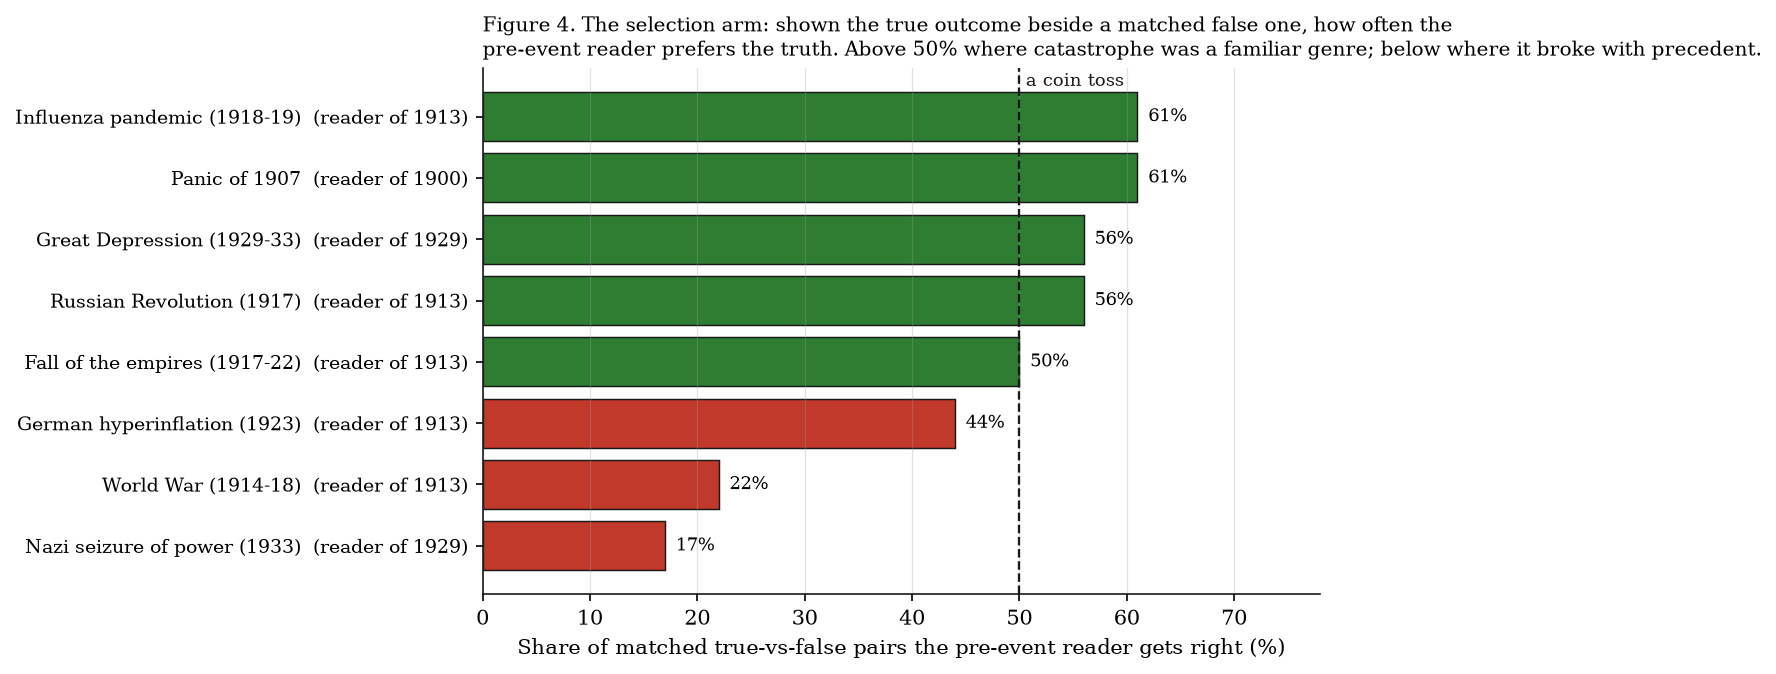
\includegraphics[width=.92\textwidth]{fig_duels.png}
\caption{The selection arm. For each event, the share of matched true-versus-false pairs the pre-event reader
gets right, pooled over the three languages; fifty per cent is a coin. Green above the line, red below.
Take-away: the pre-event reader beats the coin where catastrophe was a recurring genre and falls below it
where the event broke with precedent.}
\label{fig:duels}
\end{figure}

\begin{table}[h]\centering\small
\begin{tabular}{lrrrr}
\toprule
Event & Reader 1900 & 1913 & 1929 & Modern \\
\midrule
Nazi seizure of power (1933) & 28\% & 33\% & 17\% & 33\% \\
Panic of 1907 & 61\% & 61\% & 56\% & 50\% \\
Influenza pandemic (1918-19) & 61\% & 61\% & 44\% & 50\% \\
World War (1914-18) & 33\% & 22\% & 33\% & 28\% \\
Fall of the empires (1917-22) & 50\% & 50\% & 39\% & 39\% \\
Great Depression (1929-33) & 56\% & 50\% & 56\% & 50\% \\
Russian Revolution (1917) & 44\% & 56\% & 56\% & 39\% \\
German hyperinflation (1923) & 50\% & 44\% & 44\% & 50\% \\
\bottomrule
\end{tabular}
\caption{Forced choice between the true outcome and a matched false one: share of pairs each reader gets
right, pooled over the three languages, by event. Fifty per cent is a coin.}
\label{tab:duels}
\end{table}

\section{German and French exams}\label{app:defr}
Two runs, one declared repair between them, marks never touched. The first run failed both languages
(German \NDEfirstAnswered{}/\NexamTotal{} answered; French \NFRfirstAnswered{} answered but only
\NFRfirstOutbet{} out-bets). The repair pass fixed wording faults the autopsy traced to our side: the
German nominative bug on the Young-Turk question, the Korea-Strait second truth on Tsushima, bare
surnames for Bl\'eriot, the canonical \emph{Selbstversenkung}/\emph{sabordage} phrasings for Scapa Flow,
Compi\`egne-anchored stems for the armistice month, the missing French article on Panama, and
numbering-rule options for the French royal question (George V beside Edward VIII, Albert I, William V ---
all conceivable ex ante, so a bare-name prior no longer scores). One repair introduced its own lesson: the
reworded French Panama option did not help --- the 1929 French witness genuinely prefers Nicaragua --- and
it is counted as the wrong answer it is. Outcome: French certifies on the repaired run
(\NFRexamAnswered{} answered, \NFRexamCorrect{} right, \NFRexamOutbet{} out-bets); German fails on
coverage alone (\NDEexamAnswered{} answered, all right, \NDEexamOutbet{} out-bets) and stays uncertified.
Full per-question results for both runs are in \texttt{results/certify\_defr.json} (first run),
\texttt{results/certify\_defr\_v2.json} (repaired run), and \texttt{results/v41\_defr.json}.

\section{Abandoned designs}\label{app:graveyard}
For the record, the approaches tried and dropped, each reproducible from the results files. Surprise at a
sentence, kept as the circulation arm above, was dropped as a foresight measure once the moon scored below
bread. Averaging twenty wordings removed the noise and confirmed the null rather than rescuing it. Betting
in the future tense was dropped when the 1913 reader bet on a transatlantic tunnel and the 1929 reader, told
of the defeat, still bet on the Kaiser. Scoring only by the popularity-subtracted rule was dropped because
it drove common-phrase truths to zero; scoring only by the raw rule was dropped because it let stock phrases
win whether true or not; the two-rule agreement test is what remained. An earlier cross-model comparison
that differenced a frozen reader against a modern one was withdrawn when it proved to measure the gap between
model families rather than the gap in knowledge. On the audit side: token-probability membership tests in
the style of Min-K\% \citep{shi2024} were tried and dropped for this setting because at these corpus sizes
they are dominated by phrase frequency rather than membership; and using the memory edit to \emph{confirm}
contamination (does a planted lie overwrite more easily where nothing was stored?) returned a null ---
insertion succeeds regardless of what was there before, so edit-resistance carries no information about
prior storage. The diagnostic files are \texttt{results/diag\_square\_one.json},
\texttt{diag\_paraphrase\_pilot.json}, \texttt{diag\_betting\_pilot.json}, \texttt{diag\_retro\_pilot.json},
and \texttt{diag\_retro\_v2.json}.

\end{document}
